\documentclass[draftspec]{sbmlpkgspec}
\usepackage{tabularx}
\usepackage{tabu}
\usepackage{longtable}
\usepackage{booktabs}
\usepackage{microtype}
\usepackage{tikz}

%macros:
\newcommand{\fixttspace}{\hspace*{1pt}}

\newcommand{\sbmlthreecore}{SBML Level~3 Core\xspace}
\newcommand{\threeone}{SBML Level~3 Version~1\xspace}
\newcommand{\threetwo}{SBML Level~3 Version~2\xspace}
\newcommand{\sbmlthreedistrib}{SBML Level~3 Package Specification for Distributions, Version~1\xspace}
\newcommand{\DistributionsPackage}{\textsf{Distributions} package\xspace}
\newcommand{\TODO}[1]{\colorbox{blue}{\textcolor{white}{TODO: #1}}}

\newcommand{\DistribBase}{\defRef{DistribBase}{DistribBase-class}}
\newcommand{\UncertSpan}{\defRef{UncertSpan}{UncertSpan-class}}
\newcommand{\UncertParameter}{\defRef{UncertParameter}{UncertParameter-class}}
\newcommand{\Uncertainty}{\defRef{Uncertainty}{Uncertainty-class}}
\newcommand{\ListOfUncertainties}{\defRef{ListOfUncertainties}{ListOfUncertainties-class}}
\newcommand{\ListOfUncertParameters}{\defRef{ListOfUncertParameters}{ListOfUncertParameters-class}}


\newcommand{\ChangedMath}{\textbf{\class{ChangedMath}}\xspace}
\newcommand{\FunctionTerm}{\textbf{\class{FunctionTerm}}\xspace}
\newcommand{\LambdaClass}{\textbf{\class{Lambda}}\xspace}
\newcommand{\Math}{\textbf{\class{Math}}\xspace}
\newcommand{\QualitativeSpecies}{\textbf{\class{QualitativeSpecies}}\xspace}

\newcommand{\arraysshort}{arrays\xspace}
\newcommand{\arrays}{Arrays\xspace}
\newcommand{\distribshort}{\emph{distrib}\xspace}
\newcommand{\distrib}{Distributions\xspace}
\newcommand{\mathml}{MathML\xspace}
\newcommand{\uncertml}{UncertML\xspace}

\reversemarginpar  % Want "\watchout" to be put on the left, not the right.
\newcommand{\watchout}{\marginpar{\hspace*{34pt}\raisebox{-0.5ex}{\Large\ding{43}}}}
\newcommand{\controversial}{\marginpar{\hspace*{34pt}\raisebox{-0.5ex}{\Large?}}}
\begin{document}

\newcommand{\greencheck}{}%
\DeclareRobustCommand{\greencheck}{%
  \tikz\fill[scale=0.4, color=green]
  (0,.35) -- (.25,0) -- (1,.7) -- (.25,.15) -- cycle;%
}



\packageTitle{The Distributions Package\\for SBML Level 3}
\packageVersion{Version 1, Release 1}
\packageVersionDate{April 2, 2020}
\packageGeneralURL{http://sbml.org/Documents/Specifications/SBML_Level_3/Packages/distrib}
\packageThisVersionURL{https://co.mbine.org/specifications/sbml.level-3.version-1.distrib.version-1.release-1}

\author{%
  \begin{tabular}{c>{\hspace{20pt}}c}
  \multicolumn{2}{c}{\Large\bf{Authors}}\\
\\ Lucian P Smith           & Stuart L Moodie
\\ University of Washington & Eight Pillars Ltd
\\ Seattle, WA, USA         & Edinburgh, UK
\\
\\
  \multicolumn{2}{c}{\Large\bf{Contributors}}\\
\\ Frank Bergmann               & Colin Gillespie
\\ University of Heidelberg     & University of Newcastle
\\ Heidelberg,DE                & Newcastle, UK
\\
\\ Sarah Keating                & Matthias K\"{o}nig
\\ University College London    & Humboldt University
\\ London, UK                   & Berlin, DE
\\
\\ Chris Myers                  & Maciej J Swat
\\ University of Utah           & QSP Simcyp
\\ Salt Lake City, UT, USA      & Certara, Sheffield, UK
\\
\\ Darren Wilkinson             & Michael Hucka
\\ University of Newcastle      & California Institute of Technology
\\ Newcastle, UK                & Pasadena, CA, USA
\\
%\\
%     \multicolumn{2}{c}{Frank Bergmann}\\
%     \multicolumn{2}{c}{University of Heidelberg}\\
%     \multicolumn{2}{c}{Heidelberg, DE}\\
\end{tabular}
}

%\frontNotice{Disclaimer: This is a working draft of the SBML Level 3
%  ``distrib'' package specification. It is not a normative document.  Please
%  send comments and other feedback to the mailing list:
%  \mailto{sbml-distrib@lists.sourceforge.net.}}

\maketitlepage
\maketableofcontents


\section*{Revision History}

The following table summarizes the history of this document.

\tightspacing
\begin{table}[bh]
  \centering
  \begin{edtable}{tabularx}{\linewidth}{p{1.7cm}cp{2.3cm}X}
    \toprule
    \textbf{Version} & \textbf{Date} & \textbf{Author} & \textbf{Comments}\\
    \midrule
0.1 (Draft) & 15 Oct 2011 & Stuart Moodie & First draft \\ \midrule
0.2 (Draft) & 16 Oct 2011 & Stuart Moodie & Added introductory text
and background info. Other minor changes etc. \\ \midrule
0.3 (Draft) & 16 Oct 2011 & Stuart Moodie & Filled empty invocation
semantics section.\\ \midrule
0.4 (Draft) & 4 Jan 2012 & Stuart Moodie & Incorporated comments from
Nicolas, Maciej and Sarah. Some minor revisions and corrections.\\  \midrule
0.5 (Draft) & 6 Jan 2012 & Stuart Moodie & Incorporated addition
comments on aim of package from Nicolas.\\ \midrule
0.6 (Draft) & 19 Jul 2012 & Stuart Moodie & Incorporated revisions
discussed and agreed at HARMONY 2012.\\ \midrule
0.7 (Draft) & 6 Aug 2012 & Stuart Moodie & Incorporated review
comments from Maciej and Sarah.\\ \midrule
0.8 (Draft) & 21 Dec 2012 & Stuart Moodie & Incorporated changes
suggested at combine and subsequently through list discussions.\\ \midrule
0.9 (Draft) & 9 Jan 2013 & Stuart Moodie & Incorporated corrections
and comments from Maciej and Sarah.\\ \midrule
0.10 (Draft) & 10 Jan 2013 & Stuart Moodie & Modified based on comments
from Maciej.\\ \midrule
0.11 (Draft) & 17 May 2013 & Lucian Smith & Modified based on Stuart's proposals and PWG discussion.\\ \midrule
0.12 (Draft) & June 2013 & Lucian Smith and Stuart Moodie & Modified based on HARMONY 2013 discussion.\\ \midrule
0.13 (Draft) & July 2013 & Lucian Smith and Stuart Moodie & Modified based PWG discussion, particularly with respect to UncertML.\\ \midrule
0.14 (Draft) & March 2015 & Lucian Smith  & Modified to match UncertML 3.0.\\\midrule
0.15 (Draft) & March 2015 & Lucian Smith and Sarah Keating & Modified to match UncertML 3.0 for real this time.\\ \midrule
0.16 (Draft) & March 2015 & Lucian Smith & Added information about UncertML 3.0 distributions, and the distributions custom annotations.\\\midrule
0.17 (Draft) & June 2017 & Lucian Smith & Extensive update to reflect demise of UncertML 3.0, and appearance of ProbOnto.\\
\midrule
0.18 (Draft) & June 2017 & Lucian Smith & Fixes to reflect feedback on version 0.17.\\
\midrule
0.19 (Draft) & June 2018 & Lucian Smith & Resolved id/name issues with SBML Core L3V1 vs.\ L3V2.\\
\midrule
0.20 (Draft) & December 2018 & Lucian Smith & Updates to allow distributions as new MathML csymbols.\\
\midrule
0.21 (Draft) & January 2019 & Lucian Smith & Revisions based on suggestions from sbml-distrib, including extensive edits from Matthias.  Extended function definitions removed.\\
\midrule
0.22 (Draft) & February 2019 & Lucian Smith & Addition of \token{sampleSize} and mean values of distributions for fallback.\\
\midrule
0.23 (Draft) & February 2019 & Lucian Smith and Michael Hucka & Removal of Distribution and all subclasses; replaced with a \Math element instead; collapsed UncertStatistics into Uncertainty; some other edits.\\
\midrule
0.24 (Draft) & April 2019 & Lucian Smith & Removal of second distrib namespace, and consolidation of the \UncertParameter class based on HARMONY 2019 discussions.\\
\midrule
0.25 (Draft) & July 2019 & Lucian Smith & The \token{id} of a \UncertParameter no longer has mathematical meaning in any other context.\\
\midrule
0.26 (Release Candidate) & March 2020 & Lucian Smith & Add validation rules, and other corrections for release candidate.\\
\bottomrule
\end{edtable}
\end{table}
\regularspacing

\clearpage


\section{Introduction and motivation}

\subsection{What is the Distributions package?}

The \distrib package (also known as \distribshort) provides an extension to SBML Level 3 that extends MathML to allow draws from distributions, and also provides the ability to annotate model elements with information about the distribution their
values were drawn from. 

\subsection{Scope}

The \distrib package adds support to SBML for sampling from a
probability distribution. In particular the following are in scope:

\begin{itemize}
\item Sampling from a univariate continuous distribution
\item Sampling from a univariate discrete distribution
\item Specification of descriptive statistics (mean, standard
  deviation, standard error, etc.)
\end{itemize}

At one point the following were considered for inclusion in this
package but are now \textbf{out of scope}:

\begin{itemize}
\item Sampling from a multivariate distribution
\item Definitions of ranges as new first-order objects (the 'Arrays' package now fills that objective)
\item Sampling from user-defined probability density function
\item Stochastic differential equations
\item Other functions used to characterise a probability distribution,
  such as cumulative distribution functions (CDF) or survival functions, etc.
\end{itemize}

\subsection{This document}

This draft specification describes the consensus view of workshop participants and subscribers to the sbml-distrib mailing list. Although it was written by the listed authors, it does not solely reflect their views nor is it their proposal alone. Rather, it is their understanding of the consensus view of what the \distrib package should do and how it should do it. The contributors listed have made significant contributions to the development and writing of this specification and are credited accordingly, but a more comprehensive attribution is provided in the acknowledgments (\sec{sec:acknowledgments}).

%\subsection{Conventions used in this document}

%There are some
%parts of this draft specification where there is no clear consensus on the
%correct solution, or only recent agreement, or agreement by a group
%that may not be representative of the SBML community as a
%whole. These cases are indicated by the \controversial question mark
%in the left margin (illustrated here). The reader should pay particular
%attention to these points and ideally provide feedback, especially if
%they disagree with what is proposed. Similarly there will be points---especially as the proposal is consolidated---which are agreed,
%but which the reader should take note of and perhaps read again. These
%points \watchout are emphasized by the hand pointer in the left margin
%(illustrated).

\section{Background}

\subsection{Problems with current SBML approaches}

SBML Level 3 Core has no direct support for encoding values sampled from distributions. Currently there is no workaround within the core SBML
language itself, although it is possible to define the necessary information
using annotations on SBML elements. Frank Bergmann proposed such an annotation scheme for use with SBML Levels 2~and~3 (see \sec{sec:annotation-scheme}).

\subsection{Past work on this problem or similar topics}

\subsubsection{Newcastle Proposal 2005}
\label{sec:newcastle proposal}

In 2005, Colin Gillespie and others put forward a proposal
\footnote{\url{http://sbml.org/Community/Wiki/SBML\_Leve\l_3\_Proposals/Distributions\_and\_Ranges}}
to introduce support for probability distributions in the SBML core specification. This
was based on their need to use such distributions to represent the
models they were creating as part of the BASIS project
(\url{http://www.basis.ncl.ac.uk}).
They proposed that distributions be referred to in SBML using
the \class{csymbol} element in the \mathml subset used by
the SBML Core specification. An example is below:

\begin{example}
<math xmlns=''http://www.w3.org/1998/Math/MathML''>
  <apply>
    <csymbol encoding=''text''
        definitionURL=''http://www.sbml.org/sbml/symbols/uniformRandom''>
      uniformRandom
    </csymbol>
    <ci>mu</ci>
    <ci>sigma</ci>
  </apply>
</math>
\end{example}

This required that a library of definitions be maintained as part of
the SBML standard and in their proposal they defined an initial small
set of commonly used distributions. The proposal was never
implemented.

\subsubsection{SBML Hackathon 2010: Seattle}

The ``distrib'' package was discussed at the Seattle SBML Hackathon%
\footnote{\url{http://sbml.org/Events/Hackathons/The_2010_SBML-BioModels.net_Hackathon}}
and this section is an almost verbatim reproduction of Darren
Wilkinson's report on the
meeting\footnote{\url{http://sbml.org/Forums/index.php?t=tree\&goto=6141\&rid=0}}. In the meeting,
Darren presented an overview of the problem%
\footnote{Slides: \url{http://sbml.org/images/3/3b/Djw-sbml-hackathon-2010-05-04.pdf}}%
\footnote{Audio: \url{http://sbml.org/images/6/67/Wilkinson-distributions-2010-05-04.mov}},
building on the old proposal from the Newcastle group (see above:
\ref{sec:newcastle proposal}).  There was broad support at the meeting
for development of such a package, and for the proposed feature
set. Discussion following the presentation led to consensus on the
following points:

\begin{itemize}
\item There is an urgent need for such a package.
\item It is important to make a distinction between a description of
  uncertainty regarding a model parameter and the mechanistic process
  of selecting a random number from a probability distribution, for
  applications such as parameter scans and experimental design
\item It is probably worth including the definition of PMFs, PDFs and CDFs in the package
\item It is worth including the definition of random distributions using particle representations within such a package, though some work
 still needs to be done on the precise representation
\item It could be worth exploring the use of XML's \texttt{xinclude} construct to point at particle
representations held in a separate file
\item Random numbers must not be used in rate laws or anywhere else that
 is continuously evaluated, as then simulation behaviour is not
 defined
\item Although there is a need for a package for describing extrinsic
 noise via stochastic differential equations in SBML, such mechanisms
 should not be included in this package due to the considerable
 implications for simulator developers
\item We probably don't want to layer on top of \uncertml
 (\url{www.uncertml.org}), as this spec is fairly heavy-weight, and
 somewhat tangential to our requirements
\item A random number seed is not part of a model and should not be
 included in the package
\item The definition of truncated distributions and the specification of
 hard upper and lower bounds on random quantities should be
 considered.
\end{itemize}

It was suggested that new constructs could be introduced into SBML via user-defined functions by embedding ``distrib'' constructs in a manner illustrated by the following example:

\begin{example}
<listOfFunctionDefinitions>
  <functionDefinition id="myNormRand">
    <distrib:####>
      #### distrib binding information here ####
    </distrib:####>
    <math>
      <lambda>
        <bvar>
          <ci>mu</ci>
          <ci>sigma</ci>
        </bvar>
        <ci>mu</ci>
      </lambda>
    </math>
  </functionDefinition>
</listOfFunctionDefinitions>
\end{example}

This approach allows the use of a ``default value'' by simulators which do not
understand the package (but simulators which do will ignore the \token{<math>}
element). The package would nevertheless be ``required'', as it will not
be simulated correctly by software which does not understand the
package.

Informal discussions following the break-out covered topics such as:

\begin{itemize}
\item how to work with vector random quantities despite that SBML does not use the vector element from MathML
\item how care must be taken with the semantics of random variables
  and the need to both:
\begin{itemize}
\item reference multiple independent random quantities at a given
  time
\item make multiple references to the same random quantity at a given
time
\end{itemize}
\end{itemize}

\subsubsection{Statistical Models Workshop 2011: Hinxton}

Detailed discussion was continued at the Statistical Models Workshop
in Hinxton in June 2011%
\footnote{\url{http://sbml.org/Events/Other_Events/statistical_models_workshop_2011}}. There,
people interested in representing statistical models in SBML came
together to work out the details of how this package would work in
detail. Dan Cornford from the \uncertml
project\footnote{\url{http://www.uncertml.org/}} attended the meeting
and described how UncertML could be used to describe uncertainty
and in particular probability distributions. Perhaps the most
significant decision at this meeting was to adopt the \uncertml
resource as a controlled vocabulary that is referenced by the \distrib package.

Much has changed since this meeting, but the output from this meeting
was the basis for the first version of the ``distrib'' draft specification.


\subsubsection{HARMONY 2012: Maastricht}

Two sessions were dedicated to discussion of \distrib at HARMONY based
around the proposals described in version~0.5 of this document. In
addition there was discussion about the \arrays proposal which was
very helpful in solving the problem of multivariate distributions in
\distrib. The following were the agreed outcomes of the meeting:

\begin{itemize}
\item The original ``distrib'' draft included UncertML markup directly in the
  function definition. This proved unwieldy and confusing and has been
  replaced by a more elegant solution that eliminates the UncertML
  markup and integrates well with the fallback function (see details
  below).
\item Multivariate distributions can be supported using the \arrays
  package to define a covariance matrix.
\item User defined continuous distributions would define a PDF in
  \mathml.
\item Usage semantics were clarified so that invokation of a function
  definition implied a value was sampled from the specified
  distribution.
\item It was agreed from which sections of an SBML model a
  distribution could be invoked.
\item Statistical descriptors of variables (for
  example mean and standard deviation) would be separated from
  \distrib and either provided in a new package or in a later version
  of SBML L3 core.
\end{itemize}

\subsubsection{COMBINE 2012: Toronto}

The August draft of ``distrib'' was reviewed, and an improvement was agreed upon in
the user-defined PMF part of the proposal. In particular, is was agreed
that the categories should be defined by \distribshort classes rather
than by passing in the information as an array. Questions were also raised
about whether \uncertml was suitably well defined to be used as an
external definition for probability distributions. This was resolved
subsequent to the meeting with a teleconference to Dan Cornford and
colleagues. These changes are incorporated here. Finally, there was
considerable debate about whether to keep the dependence of
\distribshort on the Arrays package in order to support multi-variate
distributions. The outcome was an agreement that we would review this
at the end of 2012, based on the results of an investigation
into how feasible it would be to implement \arrays as a package.

\subsubsection{Package Working Group discussions 2013}

Early 2013 saw a good amount of discussion on the \distribshort Package Working Group mailing list, spurred by proposals by Stuart Moodie\footnote{\url{http://thestupott.wordpress.com/2013/03/12/an-improved-distrib-proposal/}}.  While not all of his suggestions ended up being fully accepted by the group, several changes were accepted, including:

\begin{itemize}
\item To use UncertML as actual XML, instead of as a set of reference definitions.
\item To use UncertML to encode descriptive statistics of SBML elements such as mean, standard deviation, standard error, etc.)\ bringing this capability back in scope for this package.
\end{itemize}


\subsubsection{HARMONY 2013: Connecticut}

At the HARMONY held at the University of Connecticut Health Center, further discussions revealed the importance of distinguishing the ability to describe an element as a distributed variable vs.\ a function call within the model performing a draw from a distribution.

We also decided to discard the encoding of explicit PDFs for now, as
support for it is remarkably complicated, and there no demand for
it. The current design could be extended to support this feature so if
there is demand for it in the future support for explicit PDFs could
be reintroduced.

\subsubsection{HARMONY 2017: Seattle}

In early 2017, it became clear that UncertML was no longer being worked on; the web page had lapsed, and its authors had moved on to other things.  At the same time, the ProbOnto ontology (\citealt{swat:2016}; \url{http://probonto.org/}) was developed that included all the distributions from UncertML as well as a huge number of other distributions.  On the ``distrib'' mailing list, there was discussion about whether to create essentially our own version of UncertML, or to implement a generic ``reference'' format that used ProbOnto.  The~v0.17 draft specification was developed as a compromise 'hybrid' system that did parts of both, so that basic distributions would be hard-coded, but the ability to reference any ProbOnto ontology would also be present.  The hope is that with working examples of both approaches, either the hybrid approach will be approved, or if one is preferred, the other approach may be removed.  This version of the specification was created for presentation at HARMONY 2017 in Seattle.

\subsubsection{HARMONY 2018: Oxford}

At the HARMONY held at the University of Oxford, for the first time since the change from UncertML, a libSBML implementation of the specification was available.  This let people experiment with the package, and conclude that a simpler method of defining calls to distributions was desired.  It was proposed to define new MathML \texttt{csymbol} definitions for the common distributions.  Eventually, these new \token{csymbols} were used instead of the old Distribution class, greatly simplifying the proposal.


\subsubsection{HARMONY 2019: Pasadena}

In the weeks leading up to the HARMONY held at Caltech, the PWG discussed various options for encoding uncertainties, based on different people's requirements.  At HARMONY, we were able to coalesce around an approach that seems likely to work for everyone, with multiple uncertainties per element, and a single \UncertParameter class with a \token{type} that encapsulates what used to be encoded in an element's class.


\section{Proposed syntax and semantics}

\subsection{Overview}

We use UML~1.0 (Unified Modeling Language;
\citealt{eriksson:1998, oestereich:1999}) class diagram notation to
define the constructs provided by this package.  We also use color in
the diagrams to provide additional information for the benefit of those
viewing the document on media that can display color.  The following are
the colors used and what they represent:

\begin{itemize}

\item[\raisebox{2.75pt}{\colorbox{black}{\rule{0.8pt}{0.8pt}}}]
  \emph{Black}: Items colored black in the UML diagrams are components
  taken unchanged from their definition in the SBML Level~3 Core
  specification document.

\item[\raisebox{2.75pt}{\colorbox{mediumgreen}{\rule{0.8pt}{0.8pt}}}]
  \emph{\textcolor{mediumgreen}{Green}}: Items colored green are
  components that exist in SBML Level~3 Core, but are extended by this
  package.  Class boxes are also drawn with dashed lines to further
  distinguish them.

\item[\raisebox{2.75pt}{\colorbox{darkblue}{\rule{0.8pt}{0.8pt}}}]
  \emph{\textcolor{darkblue}{Blue}}: Items colored blue are new
  components introduced in this package specification.  They have no
  equivalent in the SBML Level~3 Core specification.

\item[\raisebox{2.75pt}{\colorbox{red}{\rule{0.8pt}{0.8pt}}}]
  \emph{\textcolor{DarkRed}{Red lines}}: Classes with red lines in the corner are fully defined in a different figure.

\end{itemize}

We also use the following typographical conventions to distinguish the
names of objects and data types from other entities; these conventions
are identical to the conventions used in the SBML Level~3 Core specification
document:

\begin{description}
  
\item \abstractclass{AbstractClass}: Abstract classes are never
  instantiated directly, but rather serve as parents of other classes.
  Their names begin with a capital letter and they are printed in a
  slanted, bold, sans-serif typeface.  In electronic document formats,
  the class names defined within this document are also hyperlinked to
  their definitions; clicking on these items will, given appropriate
  software, switch the view to the section in this document containing
  the definition of that class.  (However, for classes that are
  unchanged from their definitions in SBML Level~3 Core, the class names
  are not hyperlinked because they are not defined within this
  document.)
  
\item \class{Class}: Names of ordinary (concrete) classes begin with a
  capital letter and are printed in an upright, bold, sans-serif
  typeface.  In electronic document formats, the class names are also
  hyperlinked to their definitions in this specification document.
  (However, as in the previous case, class names are not hyperlinked if
  they are for classes that are unchanged from their definitions in the
  SBML Level~3 Core specification.)

\item \token{SomeThing}, \token{otherThing}: Attributes of classes, data
  type names, literal XML, and tokens \emph{other} than SBML class
  names, are printed in an upright typewriter typeface.  Primitive types
  defined by SBML begin with a capital letter; SBML also makes use of
  primitive types defined by XML
  Schema~1.0~\citep{biron:2000,fallside:2000,thompson:2000}, but
  unfortunately, XML~Schema does not follow any capitalization
  convention and primitive types drawn from the XML~Schema language may
  or may not start with a capital letter.

\item \token{[elementName]}:  In some cases, an element may contain a child of any class inheriting from an abstract base class.  In this case, the name of the element is indicated by giving the abstract base class name in brackets, meaning that the actual name of the element depends on whichever subclass is used. The capitalization follows the capitalization of the name in brackets.

\end{description}

For other matters involving the use of UML and XML, we follow the
conventions used in the SBML Level~3 Core specification document.  


\subsection{Namespace URI and other declarations necessary for using this package}
\label{xml-namespace}

Every SBML Level~3 package is identified uniquely by an XML namespace URI.  For an SBML document to be able to use a given Level~3 package, it must declare the use of that package by referencing its URI.  This version of the \distrib package uses the URI:
\vspace*{-0.5ex}
\begin{center}
\uri{http://www.sbml.org/sbml/level3/version1/distrib/version1}
\end{center}

Note that the \distrib package may be used with both \threeone and \threetwo documents, with no semantic changes between the two in any \distribshort element, due to the addition of \token{id} and \token{name} to the \DistribBase class.

In addition, SBML documents using a given package must indicate whether the package may be used to change the mathematical meaning of \sbmlthreecore elements.  This is done using the attribute \token{required} on the \token{<sbml>} element in the SBML document.  For the \distrib package, the value of this attribute must be \val{true}, as it defines new csymbols that may be used in any MathML.  Note that the value of this attribute must \emph{always} be set to \val{true}, even if the particular model does not contain any of these csymbols.

The following fragment illustrates the beginning of a typical SBML model using \threeone and this version of the \distrib package:

\begin{example}
<?xml version="1.0" encoding="UTF-8"?>
<sbml xmlns="http://www.sbml.org/sbml/level3/version1/core" level="3" version="1"
      xmlns:distrib="http://www.sbml.org/sbml/level3/version1/distrib/version1"
      distrib:required="true">
\end{example}


The following fragment illustrates the beginning of a typical SBML model using \threetwo and this version of the \distrib package:

\begin{example}
<?xml version="1.0" encoding="UTF-8"?>
<sbml xmlns="http://www.sbml.org/sbml/level3/version2/core" level="3" version="2"
      xmlns:distrib="http://www.sbml.org/sbml/level3/version1/distrib/version1"
      distrib:required="true">
\end{example}

There is no difference between the 'distrib' part of these documents, and all package semantics are identical.

\paragraph{XML Namespace use}

For element names, XML has clear rules about how to declare and use namespaces.  In typical SBML documents, the \distrib namespace will be defined as above, and elements will therefore need to be prefixed with \val{distrib:}.

In contrast to element names, XML \emph{attribute} names are completely defined by the element in which they appear, and never have a ``default'' namespace defined. The element itself declares whether any attributes should be defined with a namespace prefix.

Following the typical convention used by SBML packages, any attribute that appears in a UML diagram in this specification may \emph{either} be defined with no namespace prefix, \emph{or} be defined with the \emph{distrib} namespace as a prefix.  (No attributes are defined here as extentions of existing core SBML elements, and thus none of them are required to have the \emph{distrib} namespace as a prefix.)


\subsection{Primitive data types}
\label{new-primitive-types}

The \distrib package uses data types described in Section~3.1 of the \sbmlthreecore specification, and adds the additional primitive types described below.

\subsubsection{Type \fixttspace\primtypeNC{ExternalRef}}
\label{sec:primtype-externalref}

The type \primtype{ExternalRef} is derived from the type \primtype{string} with the additional requirement that it be a valid URI.  An \primtype{ExternalRef} is used in the \UncertParameter class to point to ontologies such as ProbOnto~\citep{swat:2016}, which contain the definitions of distributions and parameters.

\subsubsection{Type \fixttspace\primtypeNC{UncertKind}}
\label{sec:primtype-uncertkind}

The type \primtype{UncertKind} is derived from the type \primtype{string} and its values are restricted to being one of the following possibilities: \val{coefficientOfVariation}, \val{kurtosis}, \val{mean}, \val{median}, \val{mode}, \val{sampleSize}, \val{skewness}, \val{standardDeviation}, \val{standardError}, \val{variance}, \val{confidenceInterval}, \val{credibleInterval}, \val{inter-\newline quartileRange}, \val{range}, \val{externalParameter}, and \val{distribution}.  Attributes of type \primtype{UncertKind} cannot take on any other values.  The meaning of these values is discussed in the context of the \UncertParameter class's definition in \sec{UncertParameter-class}.




\subsection{Defining Distributions}

\subsubsection{The approach}

The \distrib package has two simple purposes. First, it provides a mechanism for sampling a random value from a probability distribution. This implies that it must define the probability distribution and then must sample a random value from that distribution.  Second, it provides a mechanism for describing elements with information about their uncertainty.  An example use case for this is to provide the standard deviation for a value.  Another might be describing a parameter's distribution so it could be used in a parameter scan experiment.

Sampling from probability distributions is achieved by allowing new \mathml elements, and encoding uncertainty by extending \SBase, which in turn uses the \Uncertainty class.  Several distributions and statistics are defined explicitly in this specification, but more can be defined by referencing an external ontology such as ProbOnto through the \UncertParameter class.

%It is hoped that with this approach, modelers may use the extensions defined in this specification with a reasonable expectation that most other software packages will also recognize them.  However, if another distribution is required, those distributions may still be encoded through reference to an external ontology, even if this makes the model less exchangeable.

When a call to a distribution is defined in the extended \Math, it is sampled when it is invoked. If a particular sampled value should be used multiple times, that value must be assigned to a parameter first, such as through the use of an \InitialAssignment or \EventAssignment.  When an external distribution is defined, it is not used in the math of the model, but may be used externally where appropriate.


\begin{table}[ht]
  \centering
  \caption{The \val{definitionURL} values allowed for the \token{csymbol} of \Math for documents that use the \distribshort package, and the arguments those functions may take.}
  \vspace*{1ex}
  \begin{edtable}{tabularx}{\linewidth}{@{}>{\ttfamily}l>{\normalfont\itshape}l@{}}
\toprule
\textbf{URI} & \textbf{\textsf{\textup{Possible arguments}}} \\
\midrule
http://www.sbml.org/sbml/symbols/distrib/normal       & normal(mean, stdev) \\
                                                      & normal(mean, stdev, min, max)
\\ \midrule
http://www.sbml.org/sbml/symbols/distrib/uniform      & uniform(min, max)
\\ \midrule
http://www.sbml.org/sbml/symbols/distrib/bernoulli    & bernoulli(prob)
\\ \midrule
http://www.sbml.org/sbml/symbols/distrib/binomial     & binomial(nTrials, probabilityOfSuccess) \\
                                                      & binomial(nTrials, probabilityOfSuccess, min, max)
\\ \midrule
http://www.sbml.org/sbml/symbols/distrib/cauchy       & cauchy(scale) \\
                                                      & cauchy(location, scale) \\
                                                      & cauchy(location, scale, min, max)
\\ \midrule
http://www.sbml.org/sbml/symbols/distrib/chisquare    & chisquare(degreesOfFreedom) \\
                                                      & chisquare(degreesOfFreedom, min, max)
\\ \midrule
http://www.sbml.org/sbml/symbols/distrib/exponential  & exponential(rate)\\
                                                      & exponential(rate, min, max)
\\ \midrule
http://www.sbml.org/sbml/symbols/distrib/gamma        & gamma(shape, scale) \\
                                                      & gamma(shape, scale, min, max)
\\ \midrule
http://www.sbml.org/sbml/symbols/distrib/laplace      & laplace(scale) \\
                                                      & laplace(location, scale) \\
                                                      & laplace(location, scale, min, max) \\
\midrule
http://www.sbml.org/sbml/symbols/distrib/lognormal    & lognormal(mean, stdev) \\
                                                      & lognormal(mean, stdev, min, max)
\\ \midrule
http://www.sbml.org/sbml/symbols/distrib/poisson      & poisson(rate) \\
                                                      & poisson(rate, min, max)
\\ \midrule
http://www.sbml.org/sbml/symbols/distrib/rayleigh     & rayleigh(scale) \\
                                                      & rayleigh(scale, min, max)
\\
\bottomrule
\label{tab:csymbols}
\end{edtable}
\end{table}

\subsection{Extended \Math}
\label{sec:extended-math}

To allow quick access to a variety of common functions, the \distrib package allows the use of new types of \token{csymbol} elements anywhere that \Math is used.  These \token{csymbol}s are functions, and therefore must be the first child of an \token{apply} element, and their arguments are predefined: you cannot call \textit{normal(mean, variance)}, because the definition of the \token{normal} \token{csymbol} is \textit{normal(mean, stdev)}.

The newly-allowed \token{csymbol} elements are defined in \tab{tab:csymbols}.

Many of the distributions take exactly two or four arguments (or exactly one or three arguments).  For those functions, the optional last two arguments are \textit{min} and \textit{max}, for when the draw from the distribution is constrained to be between those two values.  For all functions, the \textit{min} boundary is inclusive; that is, a value of \textit{min} may be returned by the function (though this may be very unlikely for draws from a continuous distribution).  For all continuous distributions, the \textit{max} boundary is \emph{not} inclusive; that is, a value of \textit{max} will never be returned.  The continuous distributions are \token{normal}, \token{cauchy}, \token{chisquare}, \token{exponential}, \token{gamma}, \token{laplace}, \token{lognormal}, and \token{rayleigh}.  For the discrete distributions, the \textit{max} boundary is inclusive: that is, a value of \textit{max} may indeed be returned.  The discrete distributions are \token{binomial} and \token{poisson}.

The value of \token{min} must be less than the value of \token{max} for all continuous distributions, and the value of \token{min} must be less than or equal to the value of \token{max} for all discrete distributions.  Additionally, the \token{min} and \token{max} values of a discrete distribution must span at least one integer between them, inclusive.

To define a distribution with only one bound, the other bound should be defined as INF or -INF, as appropriate.  For those distributions that have an intrisic lower bound of 0, setting \token{min} to 0 or any negative number will have no effect, but is legal.

The versions of \token{cauchy} and \token{laplace} with one argument draw from the corresponding distribution with that argument as its scale value, and a value of \val{0} for its \token{location}.

\paragraph{Fallback functions}

If an SBML interpreter is unable to calculate one or more of the above extended \mathml functions, it may simply fail, or it might choose to return the mean of the given function instead.  In either case, it is a good idea to inform the user that the model cannot be interpreted by the software as intended. Note that the mean of a discrete distribution is not necessarily a legal return value for that function, as it may not be an integer.

The mean values in \tab{tab:meanvals} may be used as a fallback for software that cannot perform draws from a distribution.  Note that truncated versions of these functions will have different means.  Note also that the \token{cauchy} distribution has no mean, by definition.

\begin{table}[ht]
  \centering
  \caption{The mean values for the non-truncated versions of the distribution functions.  These values could potentially be used as a fallback for simulators which are not able to draw from the distributions themselves.}
  \vspace*{1ex}
  \begin{edtable}{tabularx}{4.5in}{>{\normalfont\itshape}r>{\normalfont\itshape}l}
\toprule
\textbf{\textsf{\textup{Function}}}                       & \textbf{\textsf{\textup{Fallback (mean)}}} \\ \midrule
normal(mean, stdev)                     & mean
\\ \midrule
uniform(min, max)                       & $\dfrac{\text{min}+\text{max}}{2}$
\\ \midrule
bernoulli(prob)                         & prob
\\ \midrule
binomial(nTrials, probabilityOfSuccess) & $\text{nTrials}\, \times \text{probabilityOfSuccess}$
\\ \midrule
cauchy(location, scale)                 & \textup{undefined}
\\ \midrule
chisquare(degreesOfFreedom)             & degreesOfFreedom
\\ \midrule
exponential(rate)                       & $\text{rate}^{-1}$
\\ \midrule
gamma(shape, scale)                     & $\text{shape}\, \times \text{scale}$
\\ \midrule
laplace(location, scale)                & location
\\ \midrule
lognormal(mean, stdev)                  & $\text{exp}(\text{mean} + \text{stdev}^{2}/2)$
\\ \midrule
poisson(rate)                           & rate
\\ \midrule
rayleigh(scale)                         & scale $\sqrt{\pi/2}$
\\
\bottomrule
\end{edtable}
\label{tab:meanvals}
\end{table}

\subsection{Discrete vs. continuous sampling}
\label{discrete-continuous}

\mathml csymbols may be used in \sbmlthreecore in both discrete and continuous contexts:  \InitialAssignment, \EventAssignment, \Priority, and \Delay elements are all discrete, while \Rule, \KineticLaw, and \Trigger elements are all continuous in time.  For discrete contexts, the behavior of \distribshort-extended \FunctionDefinition elements is well-defined:  a single random value is sampled from the distribution each time the function definition is invoked. Each invocation implies one sampling operation.  In continuous contexts, however, their behavior is ill-defined.  More information than is defined in this package (such as autocorrelation values or full conditional probabilities) would be required to make random sampling tractable in continuous contexts, and is beyond the scope of this version of the package.  If some package is defined in the future that adds this information, or if custom annotations are provided that add this information, such models may become simulatable.  However, this package does not define how to handle sampling in continuous contexts, and recommends against it: a warning may be produced by any software encountering the use of a \distribshort-extended \mathml in a continuous context.  Assuming such models are desirable, and the information is not provided in a separate package, this information may be incorporated into a future version of this specification.

Any other package that defines new contexts for MathML will also be either discrete or continuous.  Discrete situations (such as those defined in the SBML Level~3 Qualitative Models package) are, as above, well-defined.  Continuous situations (as might arise within the Spatial Processes package, over space instead of over time) will most likely be ill-defined.  Those packages must therefore either define for themselves how to handle \distribshort-extended \mathml elements, or leave it to some other package/annotation scheme to define how to handle the situation.



\subsection{Examples using the extended \tokenNC{csymbol} element}
\label{sec:cs-examples}

Several examples are given below that illustrate various uses of the new \token{csymbol} elements introduced by \distribshort.

\subsubsection{Using a normal distribution}

In this example, the initial value of \token{y} is set as a draw from the normal distribution $normal(z, 10)$:

\begin{example}
  <initialAssignment symbol="y">
    <math xmlns="http://www.w3.org/1998/Math/MathML">
      <apply>
        <csymbol definitionURL="http://www.sbml.org/sbml/symbols/distrib/normal"
                 encoding="text"> normal </csymbol>
        <ci> z </ci>
        <cn> 10 </cn>
      </apply>
    </math>
  </initialAssignment>
\end{example}

This use would apply a draw from a normal distribution with mean \token{z} and standard deviation \token{10} to the symbol \token{y}.

\subsubsection{Defining a truncated normal distribution}

When used with four arguments instead of two, the normal distribution is truncated to $normal(z, 10, z-2, z+2)$:

\begin{example}
  <initialAssignment symbol="y">
    <math xmlns="http://www.w3.org/1998/Math/MathML">
      <apply>
        <csymbol definitionURL="http://www.sbml.org/sbml/symbols/distrib/normal"
                 encoding="text"> normal </csymbol>
        <ci> z </ci>
        <cn type="integer"> 10 </cn>
        <apply>
          <minus/>
          <ci> z </ci>
          <cn type="integer"> 2 </cn>
        </apply>
        <apply>
          <plus/>
          <ci> z </ci>
          <cn type="integer"> 2 </cn>
        </apply>
      </apply>
    </math>
  </initialAssignment>
\end{example}

This use would apply a draw from a normal distribution with mean \token{z}, standard deviation \token{10}, lower bound \token{z $-$ 2} (inclusive) and upper bound \token{z $+$ 2} (not inclusive) to the SBML symbol \token{y}.

\subsubsection{Defining conditional events}

Simultaneous events in SBML are ordered based on their \Priority values, with higher values being executed first, and potentially cancelling events that fire after them.  In this example, two simultaneous events have priorities set with csymbols defined in \distribshort.  The event \token{E0} has a priority of $uniform(0,1)$, while the event \token{E1} has a priority of $uniform(0,2)$.  This means that 75\% of the time, event \token{E1} will have a higher priority than \token{E0}, and will fire first, assigning a value of \token{5} to parameter \token{x}.  Because this negates the trigger condition for \token{E0}, which is set \token{persistent}=\val{false}, this means that \token{E0} never fires, and the value of \token{x} remains at \token{5}.  The remaining 25\% of the time, the reverse happens, with \token{E0} setting the value of \token{x} to \token{3} instead.


\begin{example}
<?xml version="1.0" encoding="UTF-8"?>
<sbml xmlns="http://www.sbml.org/sbml/level3/version2/core"
      xmlns:distrib="http://www.sbml.org/sbml/level3/version1/distrib/version1"
      level="3" version="2" distrib:required="true">
  <model metaid="__main" id="__main">
    <listOfParameters>
      <parameter metaid="__main.x" id="x" value="0" constant="false"/>
    </listOfParameters>
    <listOfEvents>
      <event id="E0" useValuesFromTriggerTime="true">
        <trigger initialValue="true" persistent="false">
          <math xmlns="http://www.w3.org/1998/Math/MathML">
            <apply>
              <and/>
              <apply>
                <gt/>
                <csymbol encoding="text" definitionURL="http://www.sbml.org/sbml/symbols/time">
                         time </csymbol>
                <cn type="integer"> 2 </cn>
              </apply>
              <apply>
                <lt/>
                <ci> x </ci>
                <cn type="integer"> 1 </cn>
              </apply>
            </apply>
          </math>
        </trigger>
        <priority>
          <math xmlns="http://www.w3.org/1998/Math/MathML">
            <apply>
              <csymbol definitionURL="http://www.sbml.org/sbml/symbols/distrib/uniform"
                       encoding="text"> uniform  </csymbol>
              <cn type="integer"> 0 </cn>
              <cn type="integer"> 1 </cn>
            </apply>
          </math>
        </priority>
        <listOfEventAssignments>
          <eventAssignment variable="x">
            <math xmlns="http://www.w3.org/1998/Math/MathML">
              <cn type="integer"> 3 </cn>
            </math>
          </eventAssignment>
        </listOfEventAssignments>
      </event>
      <event id="E1" useValuesFromTriggerTime="true">
        <trigger initialValue="true" persistent="false">
          <math xmlns="http://www.w3.org/1998/Math/MathML">
            <apply>
              <and/>
              <apply>
                <gt/>
                <csymbol encoding="text" definitionURL="http://www.sbml.org/sbml/symbols/time">
                         time </csymbol>
                <cn type="integer"> 2 </cn>
              </apply>
              <apply>
                <lt/>
                <ci> x </ci>
                <cn type="integer"> 1 </cn>
              </apply>
            </apply>
          </math>
        </trigger>
        <priority>
          <math xmlns="http://www.w3.org/1998/Math/MathML">
            <apply>
              <csymbol definitionURL="http://www.sbml.org/sbml/symbols/distrib/uniform"
                       encoding="text"> uniform  </csymbol>
              <cn type="integer"> 0 </cn>
              <cn type="integer"> 2 </cn>
            </apply>
          </math>
        </priority>
        <listOfEventAssignments>
          <eventAssignment variable="x">
            <math xmlns="http://www.w3.org/1998/Math/MathML">
              <cn type="integer"> 5 </cn>
            </math>
          </eventAssignment>
        </listOfEventAssignments>
      </event>
    </listOfEvents>
  </model>
</sbml>
\end{example}


\begin{figure}[ht]
  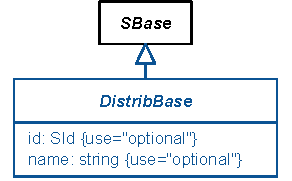
\includegraphics{figs/distribBase}
  \caption{The definition of the \DistribBase class.  The \token{id} and \token{name} attributes defined are optional, and are identical to the ones they inherit in \threetwo documents from \SBase.}
  \label{fig:distribBase}
\end{figure}

\subsection{The \class{DistribBase} class}
\label{sec:DistribBase-class}
\label{DistribBase-class}
\label{distribbase-class}
\label{sec:idname}

The \DistribBase class is an abstract base class which is the parent class for every class in this \distrib package.  Its purpose is to replicate within the \distrib package an important change between \threeone and \threetwo: the addition of an optional \token{id} and \token{name} attribute to \SBase.  By adding these attributes here, \distribshort may be used completely exchangeably between Level~3 Version~1 and Level~3 Version~2 documents without any other modifications.  The meaning of these attributes is identical, regardless of the Level/Version of the document in which they appear.

The \token{id} attribute is of type \primtype{SId}, and must be unique among other ids in the \primtype{SId} namespace in the parent \Model, and has no mathematical meaning, unless stated otherwise in the definition of that object.  The \token{name} attribute is of type \primtype{string}, and is provided to allow the user to define a human-readable label for the object.  It has no uniqueness restrictions.

\begin{figure}[ht]
  \vspace*{2em}
  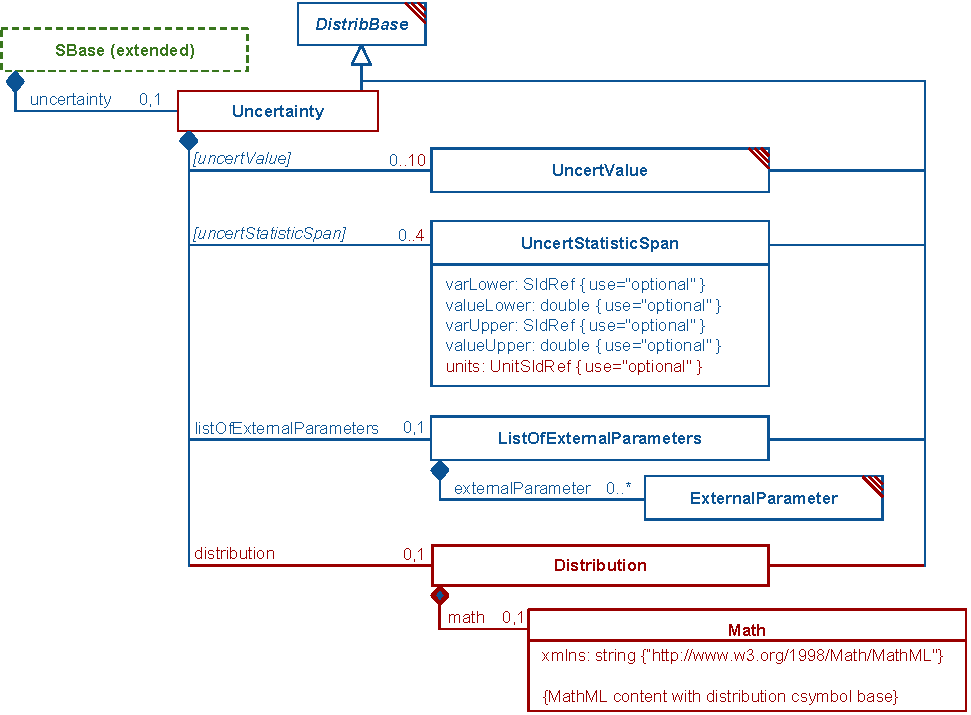
\includegraphics{figs/extended-sbase}
  \caption{The definition of the extended \SBase class to include a new optional \ListOfUncertainties child element.  Intended for use with any element with mathematical meaning, or with a \Math child element.  Also defines the \ListOfUncertainties and \Uncertainty classes.}

\label{fig:extended-sbase-uml}
\end{figure}

\subsection{The extended \SBase class}
\label{sec:extended-sbase-class}
\label{extended-sbase-class}
\label{ListOfUncertainties-class}
\label{listofuncertainties-class}

As can be seen in \fig{fig:extended-sbase-uml}, the SBML base class \SBase is extended to include an optional \ListOfUncertainties child element, which in turn contains optional \Uncertainty elements, each of which may contain a set of \UncertParameter objects that describe the uncertainty of the extended element.  Multiple \Uncertainty elements are allowed as children of \SBase to allow the modeler to record \Uncertainty measurements from different sources (papers, experiments, etc.) that may overlap and/or contradict one another.

In \sbmlthreecore, one should only extend those \SBase elements with mathematical meaning (\Compartment, \Parameter, \Reaction, \Species, and \SpeciesReference), or those \SBase elements with \Math children (\Constraint, \Delay, \EventAssignment, \FunctionDefinition, \InitialAssignment, \KineticLaw, \Priority, \Rule, and \Trigger).  The \Uncertainty child is added to \SBase instead of to each SBML element so that other packages inherit the ability to extend their own elements in the same fashion:  for example, the Qualitative Models package has the \QualitativeSpecies class which has mathematical meaning, and a \FunctionTerm class which has a \Math child.  Both could be given an \Uncertainty child containing information about the distribution or set of samples from which they were drawn.



A few SBML elements can interact in interesting ways that can confuse the semantics here.  A \Reaction element and its \KineticLaw child, for example, both reference the same mathematical formula, so only one should be extended with an \Uncertainty child element.  Similarly, the uncertainty of an \InitialAssignment will be identical to the uncertainty of the element it assigns to, and therefore only one of those elements should be extended.

Other elements not listed above should probably not be given an \Uncertainty child, as it would normally not make sense to talk about the uncertainty of something that doesn't have a corresponding mathematical meaning.  However, because packages or annotations can theoretically give new meaning (including mathematical meaning) to elements that previously did not have them, this is not a requirement.

It is important to note that the uncertainty described is defined as being the uncertainty at the moment the element's mathematical meaning is calculated, and does not describe the uncertainty of how that element changes over time.  For a \Species, \Parameter, \Compartment, and \SpeciesReference, this means that it is the uncertainty of their initial values, and does not describe the uncertainty in how those values evolve in time.  The reason for this is that other SBML constructs all describe how (or if) the values change in time, and it is those other constructs that should be used to describe a symbol's time-based uncertainty.  For example, a \Species whose initial value had uncertainty due to instrument precision could have an \Uncertainty child describing this.  A \Species whose value was known to change over time due to unknown processes, but which had a known average and standard deviation could be given an \AssignmentRule that set that \Species amount to the known average, and the \AssignmentRule itself could be given an \Uncertainty child describing the standard deviation of the variability.


\subsection{The \class{Uncertainty} class}
\label{Uncertainty-class}
\label{uncertainty-class}

The \Uncertainty class is a collection of zero or more statistical measures related to the uncertainty of the parent SBML element.  It may only contain one of each type of measurement, which means that each of its \UncertParameter children must have a unique \token{type} attribute for every value but \val{externalParameter}.  Each \UncertParameter child with a \token{type} of \val{externalParameter} must, in turn, have a unique \token{definitionURL} value.  If a given SBML element has multiple measures of the same \token{type} (for example, as measured from different sources or different experiments), it should be given multiple \Uncertainty children.  Each \Uncertainty child must be a unique set of statistical measures.

These statistical measures do not numerically affect simulation of the model.  They are, in essence, a controlled annotation format specifically designed for this sort of information.  Tools may use this information as they wish, just as they can with other annotation information.

Note that for elements that change in value over time, the described uncertainty applies only to the element's initial state, and not to how it changes in time.  For typical simulations, this means the element's initial assignment.

The child \UncertParameter children are named according to their class, so any \UncertSpan child will have the element name \token{uncertSpan}, and any \UncertParameter base class child will have the element name \token{uncertParameter}.

\paragraph{Propagation of error}

It may be possible to propagate the error defined in \Uncertainty elements through the mathematics defined in a simulation of the model.  Be advised that this will be a complicated system, and may involve calculating partial derivates of equations that are not explicitly encoded.  Many simulators choose instead to estimate the error through stochastic simulations.  Either approach should be possible with a properly encoded \distribshort model.

\clearpage

\subsubsection{Attributes inherited from \SBase}

An \Uncertainty always inherits the optional \token{metaid} and \token{sboTerm} attributes, and inherits optional \token{id} and \token{name} attributes as described in \sec{sec:idname}.  The \token{id} of an \Uncertainty has no mathematical meaning.




\begin{figure}[htb]
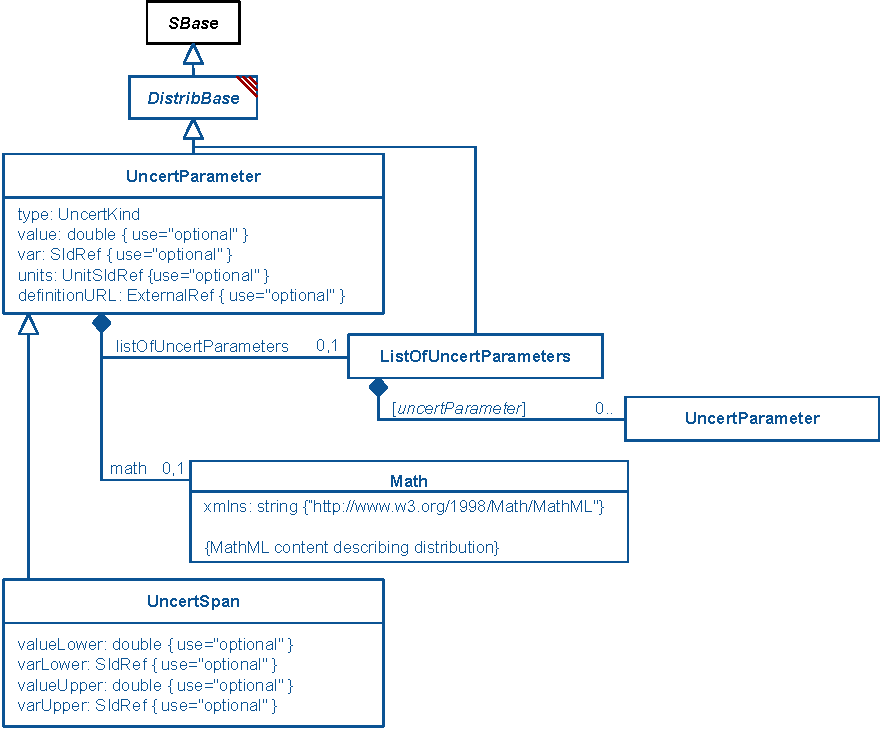
\includegraphics[width=0.85\linewidth]{figs/uncertParameter.pdf}
\caption{The definition of the \UncertParameter, \UncertSpan, and \ListOfUncertParameters classes.  These classes allow an \Uncertainty to define an uncertainty numerically.}
\label{fig:uncertParameter}
\end{figure}


\newcommand*\rot{\rotatebox{90}}

\begin{table}[ht]
  \centering
  \caption{Values for the \token{type} attribute of a \UncertParameter, the class that should be used with that type, and the attributes and children that are allowed.}
\vspace{1ex}  \begin{edtable}{tabularx}{5.2in}{>{\normalfont\itshape}X>{\normalfont\itshape}c>{\normalfont\itshape}c>{\normalfont\itshape}c>{\normalfont\itshape}c>{\normalfont\itshape}c>{\normalfont\itshape}c>{\normalfont\itshape}c>{\normalfont\itshape}c}
\toprule
\textbf{\textsf{\textup{Value}}}
& \textbf{\textsf{\textup{Class}}}
& \rot{\textbf{\textsf{\textup{units}}}}
& \rot{\textbf{\textsf{\textup{value/var}}}}
& \rot{\textbf{\textsf{\textup{valueLower/ varLower}}}}
& \rot{\textbf{\textsf{\textup{valueUpper/ varUpper}}}}
& \rot{\textbf{\textsf{\textup{definitionURL}}}}
& \rot{\textbf{\textsf{\textup{math}}}}
& \rot{\textbf{\textsf{\textup{listOfUncertParameters}}}}
\\ \midrule
coefficientOfVariation & \UncertParameter & \greencheck & \greencheck & \ding{20} & \ding{20} & \ding{20} & \ding{20} & \ding{20}
\\ \midrule
kurtosis & \UncertParameter & \greencheck & \greencheck & \ding{20} & \ding{20} & \ding{20} & \ding{20} & \ding{20}
\\ \midrule
mean & \UncertParameter & \greencheck & \greencheck & \ding{20} & \ding{20} & \ding{20} & \ding{20} & \ding{20}
\\ \midrule
median & \UncertParameter & \greencheck & \greencheck & \ding{20} & \ding{20} & \ding{20} & \ding{20} & \ding{20}
\\ \midrule
mode & \UncertParameter & \greencheck & \greencheck & \ding{20} & \ding{20} & \ding{20} & \ding{20} & \ding{20}
\\ \midrule
sampleSize & \UncertParameter & \greencheck & \greencheck & \ding{20} & \ding{20} & \ding{20} & \ding{20} & \ding{20}
\\ \midrule
skewness & \UncertParameter & \greencheck & \greencheck & \ding{20} & \ding{20} & \ding{20} & \ding{20} & \ding{20}
\\ \midrule
standardDeviation & \UncertParameter & \greencheck & \greencheck & \ding{20} & \ding{20} & \ding{20} & \ding{20} & \ding{20}
\\ \midrule
standardError & \UncertParameter & \greencheck & \greencheck & \ding{20} & \ding{20} & \ding{20} & \ding{20} & \ding{20}
\\ \midrule
variance & \UncertParameter & \greencheck & \greencheck & \ding{20} & \ding{20} & \ding{20} & \ding{20} & \ding{20}
\\ \midrule
confidenceInterval & \UncertSpan & \greencheck & \ding{20} & \greencheck & \greencheck & \ding{20} & \ding{20} & \ding{20}
\\ \midrule
credibleInterval & \UncertSpan & \greencheck & \ding{20} & \greencheck & \greencheck & \ding{20} & \ding{20} & \ding{20}
\\ \midrule
interquartileRange & \UncertSpan & \greencheck & \ding{20} & \greencheck & \greencheck & \ding{20} & \ding{20} & \ding{20}
\\ \midrule
range & \UncertSpan & \greencheck & \ding{20} & \greencheck & \greencheck & \ding{20} & \ding{20} & \ding{20}
\\ \midrule
distribution & \UncertParameter  & \greencheck & \ding{20} & \ding{20} & \ding{20} & \greencheck & \greencheck & \greencheck
\\ \midrule
externalParameter & either & \greencheck & \greencheck & \greencheck & \greencheck & \greencheck & \greencheck & \greencheck
\\
\bottomrule
\label{tab:uncertparamtype}
\end{edtable}
\end{table}

\subsection{The \class{UncertParameter} class}
\label{ListOfUncertParameters-class}
\label{listofuncertparameters-class}
\label{UncertParameter-class}
\label{uncertparameter-class}

Each \UncertParameter defines one uncertainty statistic about the parent element.  It has one required attribute \token{type} of type \primtype{UncertKind} which defines what statistic it describes (i.e. \val{mean}, \val{standardDeviation}, \val{distribution}, etc.).  Its other attributes (\token{value}, \token{var}, \token{units}, and \token{definitionURL}), and children (\token{math} and \token{list\-Of\-Uncert\-Pa\-ra\-me\-ters}) are all optional, each useable according to which \token{type} it is.

\subsubsection{The \token{type} attribute}
The \token{type} attribute defines what the \UncertParameter describes.  Depending on the type, other attributes will be allowed or not, and the class must either be the base \UncertParameter or the \UncertSpan class, according to \tab{tab:uncertparamtype}.


\subsubsection{The \token{value} and \token{var} attributes}
The optional \token{value} attribute (of type \primtype{double}) is used when the \UncertParameter equals the given number, and the optional \token{var} attribute (of type \primtype{SIdRef}) is used when the value of an \UncertParameter equals the referenced element with mathematical meaning.  Either attribute may be used for those \UncertParameter types with a single value, but not both.

\subsubsection{The \token{units} attribute}
The optional \token{units} attribue of an \UncertParameter is of type \primtype{UnitSIdRef}.  The \primtype{UnitSIdRef} is defined in the \sbmlthreecore specification, but in brief, it may either be the \primtype{SId} of a \UnitDefinition in the \Model, or a predefined SI unit from the Table~2 in the \sbmlthreecore specification.  The units of uncertainty statistics are generally either dimensionless or the same as the units of the parent, according to the formula that defines the value.  A \token{mean} and a \token{standardDeviation}, for example, are always the same units as the parent, while a \token{coefficientOfVariation} is dimensionless.

\subsubsection{The \token{definitionURL} attribute}
The optional \token{definitionURL} attribute (of type \primtype{ExternalRef}) may be used when the \token{type} of the \UncertParameter is \val{distribution}, and must be used when the \token{type} of the \UncertParameter is \val{externalParameter}.  The \primtype{ExternalRef} should point to an ontology URL, distribution \token{csymbol}, or other unique definition string that defines what is meant by this \UncertParameter.  The \token{definitionURL} must not be defined if the \token{type} is any other value: the other types are already completely defined.

\subsubsection{Attributes inherited from \SBase}
An \UncertParameter always inherits the optional \token{metaid} and \token{sboTerm} attributes, and inherits optional \token{id} and \token{name} attributes as described in \sec{sec:idname}.  The \token{id} of a \UncertParameter does not take on the mathematical value of its \token{value} attribute, and may not be used in mathematical contexts.  Instead, if the value of the element is to be used elsewhere, the \token{var} attribute should be used instead, and that referenced value used in other contexts.

\subsubsection{The child \token{math} element}
The optional \token{math} element contains MathML, and may only be used for an \UncertParameter of type \val{distribution} or \val{externalParameter}.  When defined for a \val{distribution}, the MathML should define that distribution, such as by using one of the extended \token{csymbol} definitions from this specification.

\subsubsection{The child \token{ListOfUncertParameters} element}
The optional child \token{ListOfUncertParameters} element may only be used for an \UncertParameter of type \val{dist\-ri\-bu\-tion} or \val{externalParameter}.  Unlike an \Uncertainty, there are no uniqueness restrictions among the children of this element: any number of \UncertParameter elements of any \token{type} may be used, according to whatever makes sense for the statistic defined by the parent \token{definitionURL}.

\subsection{The \class{UncertSpan} class}
\label{UncertSpan-class}
\label{uncertspan-class}

The \UncertSpan class defines a span of values that define an uncertainty statistic such as confidence interval or range.  It inherits from \UncertParameter, and adds four optional attributes, \token{varLower} and \token{varUpper}, of type \primtype{SIdRef}, and \token{valueLower} and \token{valueUpper}, of type \primtype{double}.  Exactly one of the attributes \token{varLower} and \token{valueLower} may be defined, and exactly one of the attributes \token{varUpper} and \token{valueUpper} may be defined.  If no attributes are defined, the parameters of the span are undefined.  If only one attribute is defined (one of the upper or lower attributes), that aspect of the span is defined, and the other end is undefined.  The span is fully defined if two attributes (one lower and one upper) are defined.

The value of the lower attribute (whichever is defined) must be lesser or equal to the value of the upper attribute (whichever is defined), at the initial conditions of the model.  The \Uncertainty element cannot affect the core mathematics of an SBML model, but if it is used in a mathematical context during simulation of the model, this restriction on the attribute values must be maintained, or the \UncertSpan object as a whole will be undefined.

Like the \token{units} attribute on an \UncertParameter, the \token{units} attribute is provided if \token{valueUpper} and/or \token{valueLower} is defined.  The units on both the upper and lower ends of the span must match each other, if defined.  The units for span ends defined by reference may be obtained from the referenced SBML element.




\subsection{The different \class{UncertParameter} and \class{UncertSpan} \token{type} values.}

The \primtype{UncertKind} values each have a particular definition.  The following kinds are all single-value types, and thus may either be defined by \token{value} or \token{var}, and must only be used for \UncertParameter elements, not \UncertSpan elements.  Definitions taken from \url{https://web.archive.org/web/20161029215725/uncertml.org/}).


\begin{itemize}

\item \token{coefficientOfVariation}:  For a random variable with mean $ \mu $ and strictly positive standard deviation $ \sigma $, the coefficient of variation is defined as the ratio $ \frac{\sigma}{\mid\mu\mid} $. One benefit of using the coefficient of variation rather than the standard deviation is that it is unitless.

\item \token{kurtosis}:  The kurtosis of a distribution is a measure of how peaked the distribution is. The kurtosis is defined as $ \mu_4/\sigma^4 $ where $ \mu_4 $ is the fourth central moment of the distribution and $ \sigma $ is its standard deviation.

\item \token{mean}:  The arithmetic mean (typically just the mean) is what is commonly called the average. It is defined as $ \bar{x} = \frac{1}{n}\cdot \sum_{i=1}^n{x_i} $ where $ x_i $ represents with $ i $th observation of the quantity $ x $ in the sample set of size $ n $. It is related to the expected value of a random variable, $ \mu = E[X] $ in that the population mean, $ \mu $, which is the average of all quantities in the population and is typically not known, is replaced by its estimator, the sample mean $ \bar{x} $. Note that this statistic does not deal with issues of sample size, rather the mean is taken to refer to the population mean.

\item \token{median}:  The median is described as the numeric value separating the higher half of a sample (or population) from the lower half. The median of a finite list of numbers can be found by arranging all the observations from lowest value to highest value and picking the middle one. If there is an even number of observations, then there is no single middle value, then the average of the two middle values is used. The median is also the 0.5 quantile, or 50th percentile.

\item \token{mode}:  The mode is the value that occurs the most frequently in a data set (or a probability distribution). It need not be unique (e.g., two or more quantities occur equally often) and is typically defined for continuous valued quantities by first defining the histogram, and then giving the central value of the bin containing the most counts.

\item \token{sampleSize}:  The sample size is a direct count of the number of observations made or the number of samples measured.  It is used in several other statistical measurements, and can be used to convert one to another.

\item \token{skewness}:  The skewness of a random variable is a measure of how asymmetric the corresponding probability distribution is. The skewness is defined as $ \mu_3/\sigma^3 $ where $ \mu_3 $ is the 3rd central moment of the distribution and $ \sigma $ is its standard deviation.

\item \token{standardDeviation}:  The standard deviation of a distribution or population is the square root of its variance and is given by $ \sigma = \sqrt{E[(X - \mu)^2]} $ where $ \mu = E[X] $. The population standard deviation is given by $ \sigma = \sqrt{\frac{1}{n} \sum_{i=1}^n\left(x_i - \bar{x} \right)^2} $ where $ \bar{x} = \frac{1}{n}\cdot \sum_{i=1}^n{x_i} $, and $ x_i $ represents the $ i $th observation of the quantity $ x $ in the population of size $ n $. The standard deviation is a widely used measure of the variability or dispersion since it is reported in the natural units of the quantity being considered. Note that if a finite sample of a population has been used then the sample standard deviation is the appropriate unbiased estimator to use.

\item \token{standardError}:  The standard error is the standard deviation of estimates of a population value. If that population value is a mean, this statistic is called the standard error of the mean.  It is calculated as the standard deviation of a sample divided by the square root of the number of the sample size.  As the sample size increases, the sample size draws closer to the population size, and the standard error approaches zero.  $ \sigma_{\bar{x}} = \sigma/\sqrt{n} $.

\item \token{variance}:  The variance of a random quantity (or distribution) is the average value of the square of the deviation of that variable from its mean, given by $ \sigma^2 = \text{Var}[X] = E[(X - \mu)^2] $ where $ \mu = E[X] $. The complete population variance is given by $ \sigma^2 = \frac{1}{n} \sum_{i=1}^n\left(x_i - \bar{x} \right)^2 $ where $ \bar{x} = \frac{1}{n}\cdot \sum_{i=1}^n{x_i} $, and $ x_i $ represents the $ i $th observation of the quantity $ x $ in the population of size $ n $. This is the estimator of the population variance and should be replaced by the sample variance when using samples of finite size.

\end{itemize}

The following \token{UncertKind} values are all spans, and may only be used for \UncertSpan elements.  They are defined by an upper and lower value.  Definitions taken from taken from \url{https://web.archive.org/web/20161029215725/uncertml.org/}).

\begin{itemize}

\item {\token{confidenceInterval}:  For a univariate random variable $ x $, a confidence interval is a range $ [a,b] $, $ a<b $, so that $ x $ lies between $ a $ and $ b $ with given probability. For example, a 95\% confidence interval is a range in which $ x $ falls 95\% of the time (or with probability 0.95). Confidence intervals provide intuitive summaries of the statistics of the variable $ x $.

If $ x $ has a continuous probability distribution $ P $, then $ [a,b] $ is a 95\% confidence interval if $ \int_a^b P(x) = 0.95 $.

Unless specified otherwise, the confidence interval is usually chosen so that the remaining probability is split equally, that is $ P(x<a) = P(x>b) $. If $ x $ has a symmetric distribution, then the confidence intervals are usually centered around the mean. However, non-centered confidence intervals are possible and are better described by their lower and upper quantiles or levels. For example, a 50\% confidence interval would usually lie between the 25\% and 75\% quantiles, but could in theory also lie between the 10\% and 60\% quantiles, although this would be rare in practice. The \token{confidenceInterval} allows you the flexibility to specify non-symmetric confidence intervals however in practice we would expect the main usage to be for symmetric intervals.

The \token{confidenceInterval} child of a \Uncertainty is always the 95\% confidence interval.  For other confidence intervals, use an \UncertParameter of type \val{externalParameter} instead. }

\item {\token{credibleInterval}:  In Bayesian statistics, a credible interval is similar to a confidence interval determined from the posterior distribution of a random variable $ x $. That is, given a prior distribution $ p(x) $ and some observations $ D $, the posterior probability $ p(x\mid D) $ can be computed using Bayes theorem. A 95\% credible interval is then any interval $ [a,b] $ so that $ \int_a^b p(x\mid D) = 0.95 $, that is the variable $ x $ lies in the interval $ [a,b] $ with posterior probability 0.95. Note that the interpretation of a credible interval is not the same as a (frequentist) confidence interval.

The \token{credibleInterval} child of a \Uncertainty is always the 95\% credible interval.  For other credibility intervals, use an \UncertParameter of type \val{externalParameter} instead.}


\item \token{interquartileRange}:  The interquartile range is the range between the 1st and 3rd quartiles. It contains the middle 50\% of the sample realisations (or of the sample probability). It is typically used and shown in box plots.

\item \token{range}:  The range is the interval $ [a,b] $ so that $ a<b $ and contains all possible values of $ x $. This is also often called the statistical range, which is the distance from the smallest value to the largest value in a sample dataset. For a sample dataset $ X = (x_1, ..., x_N $), the range is the distance from the smallest $ x_i $ to the largest. It is often used as a first estimate of the sample dispersion.

\end{itemize}

Finally, we have the \val{distribution} and \val{externalParameter} types:

\begin{itemize}

\item {\token{distribution}}: If the uncertainty is defined by a known distribution, that distribution may either be defined by using the child \token{math} element, or by using the \token{definitionURL}.  When the \token{math} child is used, that math should contain the distribution in question:  typically this will be a distribution \token{csymbol} but may be something more complicated, like a \token{piecewise} function.  If the \token{definitionURL} is used, many more distributions may be used than are defined in this specification (like an \token{externalParameter}, below).  To fully define this distributon, it will almost certainly be necessary to further define that distribution with child \UncertParameter elements.  For example, a Beta distribution takes two parameters ($\alpha$ and $\beta$), each of which could be defined by a child \UncertParameter of type \val{externalParameter}, with appropriate \token{definitionURL} values.  A \token{type} of value \val{distribution} is only valid for \UncertParameter elements, not \UncertSpan elements.

\item{\token{externalParameter}}: This type is uniquely described by an appropriate \token{definitionURL}, and is provided to allow a modeler to encode externally-provided parameters not otherwise explicitly handled by this specification.  The range of possibilities is vast, so modelers should ensure that the tool they wish to use encodes support for any \UncertParameter they define.  As an external parameter may take any form, there are no restrictions on what other attributes or children that may be used by an \UncertParameter of this type:  it may be a single value; it may be a span; it may be defined by a child \token{math} element; it may be defined by child \UncertParameter elements; it may be defined by any combination of the above.  The only restriction is that the \token{definitionURL} \emph{must} be defined for any \UncertParameter of type \val{externalParameter}.  This type value may be used for either \UncertParameter or \UncertSpan elements.

As an example, here's an \UncertSpan that defines the 99\% confidence interval of a \Parameter (using made-up \token{definitionURL} values):

\begin{example}
  <parameter id="p1" value="3.42" constant="true">
    <distrib:listOfUncertainties>
      <distrib:uncertainty>
        <distrib:uncertSpan type="externalParameter" lowerValue="3.19" upperValue="3.83"
                            definitionURL="http://dist.org/CI">
          <distrib:listOfUncertParameters>
            <distrib:uncertParameter type="externalParameter" value="0.99"
                            definitionURL="http://dist.org/CIpercent">
          </distrib:listOfUncertParameters>
        </distrib:uncertSpan>
      </distrib:uncertainty>
    </distrib:listOfUncertainties>
  </parameter>
\end{example}

\end{itemize}

As examples, the following statistics are not defined by a single value nor by a range, and would therefore be good candidates for encoding as an external parameter.  These terms were included in the now-defunct UncertML (and the definitions were again taken from \url{https://web.archive.org/web/20161029215725/uncertml.org/}), and may also be findable in other ontologies such as STATO (which has a searchable database at \url{https://www.ebi.ac.uk/ols/ontologies/stato}):

\begin{itemize}
\item \token{centralMoment}:  For a given positive natural number $ k $, the $ k\textsuperscript{th} $ central moment of a random variable $ x $ is defined as $ \mu_k = E[(x - E[x])^k] $. That is, it is the expected value of the deviation from the mean to the power $ k $. In particular, $ \mu_0 = 1 $, $ \mu_1 = 0 $ and $ \mu_2 $ is the variance of $ x $.

\item \token{correlation}:  The correlation between two random variables $ x_1 $ and $ x_2 $ is the extent to which these variable vary together in a linear fashion. It is characterized by the coefficient $ \rho_{1,2} = E[(x_1-\mu_1)(x_2-\mu_2)] / \sigma_1\sigma_2 $ where $ \mu_1 $ and $ \mu_2 $ are the means of $ x_1 $ and $ x_2 $ respectively, and $ \sigma_1 $ and $ \sigma_2 $ are their respective standard deviations. Note this is strictly not a description of uncertainty, but it can be useful to represent the correlation between two variables. Generally a covariance specification would be preferred since this describes the uncertainty.

\item \token{decile}:  A decile, $ d $, is any of the nine values that divide the sorted quantities into ten equal parts, so that each part represents 1/10 of the sample, population or distribution. The first decile is equivalent to the 10th percentile.

\item \token{moment}:  For a given positive natural number $ k $, the $ k\textsuperscript{th} $ moment of a random variable $ x $ is defined as $ \mu_k = E[x^k] $. In particular, $ \mu_0 = 1 $ and $ \mu_1 $ is the mean of $ x $.
The moments can be defined with respect to some point $ a $, that is $ \mu_k(a) = E[(x - a)^k] $. Moments defined about the mean are called central moments.

\item \token{percentile}:  A percentile is the value of a quantity below which a certain percent of values fall. This can be defined for samples, populations and distributions. For finite samples there is no widely accepted method, but all methods essentially rank the quantities and then use some interpolation to compute the percentile, unless the sample size $ n $ is a multiple of 100. For probability distributions the inverse cumulative density function can be used.  The most widely used method is as follows: to estimate the value, $ x_p $, of the $ p $th percentile of an ascending ordered dataset containing $ n $ elements with values $ x_1, x_2, ... ,x_n $ first compute $ \rho = \frac{p}{100}\,({n}-1)+1 $. Now $ \rho $ is split into its integer component, $ k $, and decimal component, $ d $, such that $ \rho = k + d $. $ x_p $ is then calculated as $ x_p = x_k+d(x_{k+1}-x_k) $ where $ 1 < \rho < n $ with special cases $ x_p = x_1 \; [\rho=1]; \ x_n \; [\rho=n] $.

\item \token{probability}:  Given a random variable $ x $ with probability density function $ f(x) $, the probability that $ x $ lies in some part of its domain $ \mathcal{X} $ is defined as $ P(x \in \mathcal{X}) = \int_{x\in\mathcal{X}} f(x) $. $ \mathcal{X} $ can be defined as a lower- or upper-bounded range, e.g., $ P(x < 3.2) $, or as the intersection of several such ranges, e.g., $ P(x \geq 1.7 \cap x < 3.2) $.

\item \token{quantile}:  Given a random variable $ x $, the $ n $-quantiles are the values of $ x $ which split the domain into $ n $ regions of equal probability. For instance, the $ k\textsuperscript{th} $ $ n $-quantile is the value $ q_k $ for which $ P(x<q_k) = \frac{k}{n} $. For some common values of $ n $, the $ n $-quantiles have additional names, namely quartiles for $ n=4 $, deciles for $ n=10 $ and percentiles for $ n=100 $.
More generally, a quantile can be associated to any probability $ p $, so that $ q $ is the value of $ x $ below which a proportion $ p $ of the probability lies, i.e., $ P(x<q) = p $.
The plot on the right shows the 1st to 9th 10-quantiles (or deciles) for a normal distribution ($ \mu = 4 $, $ \sigma = 1 $) as orange dots. The blue curve is the cumulative density function of $ x $. Note how the quantiles split the probability (y-axis) into 10 equal regions.

\item \token{quartile}:  The quartiles are the 4-quantiles, that is the 4 values of $ x $ below which lies a proportion 0.25, 0.50, 0.75 and 1 of the probability. One can also think of them as the 4 values of $ x $ which split the domain into 4 regions of equal probability.
\end{itemize}




\subsection{The uncertainty of a \Species}

A \Species is a unique SBML construct in that its value is either an amount or a concentration, depending on the value of its \token{hasOnlySubstanceUnits} attribute (\val{true} for amount, or \val{false} for concentration).  The value of its uncertainty tracks with this: if the value of \token{hasOnlySubstanceUnits} on the parent \Species is \val{true}, the uncertainty is in terms of amounts, and if \val{false}, the uncertainty is in terms of concentration.

If a \Species is being modeled in SBML in amounts, but was measured in terms of its concentration, or visa versa, an \InitialAssignment should be created that explicitly handles this conversion and assigns the appropriate value to the \Species, as in the example below.

%\clearpage

\begin{example}
    <listOfCompartments>
      <compartment id="C" spatialDimensions="3" size="2" constant="true">
        <distrib:listOfUncertainties>
          <distrib:uncertainty>
            <distrib:uncertParameter type="standardDeviation" value="0.15"/>
          </distrib:uncertainty>
        </distrib:listOfUncertainties>
      </compartment>
    </listOfCompartments>
    <listOfSpecies>
      <species id="S_amt" compartment="C" hasOnlySubstanceUnits="true"
               boundaryCondition="false" constant="false"/>
    </listOfSpecies>
    <listOfParameters>
      <parameter id="S_conc" value="3.4" constant="true">
        <distrib:listOfUncertainties>
          <distrib:uncertainty>
            <distrib:uncertParameter type="standardDeviation" value="0.3"/>
          </distrib:uncertainty>
        </distrib:listOfUncertainties>
      </parameter>
    </listOfParameters>
    <listOfInitialAssignments>
      <initialAssignment symbol="S_amt">
        <math xmlns="http://www.w3.org/1998/Math/MathML">
          <apply>
            <times/>
            <ci> S_conc </ci>
            <ci> C </ci>
          </apply>
        </math>
      </initialAssignment>
    </listOfInitialAssignments>
\end{example}

Here, the uncertainty of the species \val{S\_amt} is not set explicitly, and instead can be derived from the uncertainty of the values in its initial assignment (\val{S\_conc} and \val{C}).



\clearpage

\subsection{Examples using \class{Uncertainty}}
\label{extended-sbase-examples}

Several examples are given to illustrate the use of the \Uncertainty class:


\subsubsection{Basic \Uncertainty example}

In this examples, a species is given an \Uncertainty child to describe its standard deviation:

\begin{example}
  <species id="s1" compartment="C" initialAmount="3.22" hasOnlySubstanceUnits="true"
           boundaryCondition="false" constant="false">
    <distrib:listOfUncertainties>
      <distrib:uncertainty>
        <distrib:uncertParameter type="standardDeviation" distrib:value="0.3"/>
      </distrib:uncertainty>
    </distrib:listOfUncertainties>
  </species>
\end{example}
\vspace*{1.5ex}

Here, the species with an initial amount of 3.22 is described as having a standard deviation of 0.3, a value that might be written as \val{3.22 $\pm$ 0.3}.  This is probably the simplest way to use the package to introduce facts about the uncertainty of the measurements of the values present in the model.

It is also possible to include additional information about the species, should more be known:

\begin{example}
  <species id="s1" compartment="C" initialAmount="3.22" hasOnlySubstanceUnits="true"
           boundaryCondition="false" constant="false">
    <distrib:listOfUncertainties>
      <distrib:uncertainty>
        <distrib:listOfUncertParameters>
          <distrib:uncertParameter type="mean" distrib:value="3.2"/>
          <distrib:uncertParameter type="standardDeviation" distrib:value="0.3"/>
          <distrib:uncertParameter type="variance" distrib:value="0.09"/>
        </distrib:listOfUncertParameters>
      </distrib:uncertainty>
    </distrib:listOfUncertainties>
  </species>
\end{example}

In this example, the initial amount of 3.22 is noted as having a mean of 3.2, a standard deviation of 0.3, and a variance of 0.09.  Note that the standard deviation can be calculated from the variance (or visa versa), but the modeler has chosen to include both here for convenience.  Note too that this use of the \Uncertainty element does not imply that the species amount comes from a normal distribution with a mean of 3.2 and standard deviation of 0.3, but rather that the species amount comes from an unknown distribution with those qualities.  If it is known that the value was drawn from a particular distribution, an \UncertParameter of type \val{distribution} should be used, rather than \UncertParameter elements of type \val{mean} and \val{standardDeviation}.

Note also that 3.22 (the \token{initialAmount}) is different from 3.2 (the \token{mean}):  evidently, this model was constructed as a realization of the underlying uncertainty, instead of simply using the mean.


\subsubsection{Defining a random variable}

In addition to describing the uncertainty about an experimental
observation one can also use this mechanism to describe a parameter as
a random variable. In the example below the parameter, \token{Z}, is defined
as following a gamma distribution, with a given shape and scale. No
value is given for the parameter so it is then up the modeler to
decide how to use this random variable. For example they may choose to
simulate the model in which case they may provide values for \token{shape\_Z}
and \token{scale\_Z} and then sample a random value from the
simulation. Alternatively they may choose to carry out a parameter
estimation and use experimental observations to estimate \token{shape\_Z} and
\token{scale\_Z}.

For added information, the modeler has chosen to include the observed mean and variance of the value.  These are close to the expected mean and variance from the given distribution (1.0 and 0.1, respectively, given the shape and scale), but were slightly different due to the sample size.

\begin{example}
<listOfParameters>
  <parameter id="shape_Z" value="10" constant="true"/>
  <parameter id="scale_Z" value="0.1" constant="true"/>
  <parameter id="Z" constant="true">
    <distrib:listOfUncertainties>
      <distrib:uncertainty>
        <distrib:uncertParameter type="distribution">
          <math xmlns="http://www.w3.org/1998/Math/MathML">
            <apply>
              <csymbol definitionURL="http://www.sbml.org/sbml/symbols/distrib/gamma"
                       encoding="text"> gamma </csymbol>
              <ci> shape_Z </ci>
              <ci> scale_Z </ci>
            </apply>
          </math>
        </distrib:uncertParameter>
        <distrib:uncertParameter type="mean" value="1.03"/>
        <distrib:uncertParameter type="variance" value="0.97"/>
      </distrib:uncertainty>
    </distrib:listOfUncertainties>
  </parameter>
</listOfParameters>
\end{example}

\subsubsection{Defining external distributions}
\label{sec:external-dist-example}

If an SBML value is drawn from a distribution not defined explicitly in this specification, it is necessary to use an \UncertParameter of type \val{externalParameter} to define the distribution's parameters.  In this example, the parameter \token{p1} was drawn from a zeta distribution, with a shape parameter of 2.37.  An \UncertParameter of type \val{distribution} is created with the 'zeta' URI, with a child \UncertParameter of type \val{externalParameter} with the 'shape' URI for its \token{definitionURL}.  For readability, 'zeta' and 'shape' were used as the names of these parameters.


\begin{example}
<parameter id="p1" constant="true">
  <listOfUncertainties xmlns="http://www.sbml.org/sbml/level3/version1/distrib/version1">
    <uncertainty>
      <uncertParameter type="distribution" name="zeta"
                 definitionURL="http://www.probonto.org/ontology#PROB_k0001263">
        <listOfUncertParameters>
          <uncertParameter type="externalParameter" name="shape" value="2.37"
                 definitionURL="http://purl.obolibrary.org/obo/STATO_0000436"/>
        </listOfUncertParameters>
      </uncertParameter>
    </uncertainty>
  </listOfUncertainties>
</parameter>
\end{example}


It is also possible to create even more complex structures with the \UncertParameter scheme.  In this example, we define a categorical distribution based on data from three patients.  The parent \UncertParameter is defined to be the 'categorical' distribution, with three 'category' children, each with two child 'value' and 'probability' parameters.  Collectively, they define a distribution where a value of 1.01 has a probability of 50\%, a value of 2.24 has a probability of 25\%, and a value of 1.72 has a probability of 25\%.  (The \token{definitionURL} examples here were made up for the purposes of this example, to be readable.  In an actual SBML document, they would point to existing external ontologies.)

\clearpage

\begin{example}
<listOfUncertainties xmlns="http://www.sbml.org/sbml/level3/version1/distrib/version1">
  <uncertainty>
    <listOfUncertParameters>
      <uncertParameter type="distribution" definitionURL="http://dist.org/categorical">
        <listOfUncertParameters>
          <uncertParameter type="externalParameter" id="p1" definitionURL="http://dist.org/category">
            <listOfUncertParameters>
              <uncertParameter type="externalParameter" value="1.01"
                               definitionURL="http://dist.org/cat_val"/>
              <uncertParameter type="externalParameter" value="0.5"
                               definitionURL="http://dist.org/cat_prob"/>
            </listOfUncertParameters>
          </uncertParameter>
          <uncertParameter type="externalParameter" id="p2" definitionURL="http://dist.org/category">
            <listOfUncertParameters>
              <uncertParameter type="externalParameter" value="2.24"
                               definitionURL="http://dist.org/cat_val"/>
              <uncertParameter type="externalParameter" value="0.25"
                               definitionURL="http://dist.org/cat_prob"/>
            </listOfUncertParameters>
          </uncertParameter>
          <uncertParameter type="externalParameter" id="p3" definitionURL="http://dist.org/category">
            <listOfUncertParameters>
              <uncertParameter type="externalParameter" value="1.72"
                               definitionURL="http://dist.org/cat_val"/>
              <uncertParameter type="externalParameter" value="0.25"
                               definitionURL="http://dist.org/cat_prob"/>
            </listOfUncertParameters>
          </uncertParameter>
        </listOfUncertParameters>
      </uncertParameter>
    </listOfUncertParameters>
  </uncertainty>
</listOfUncertainties>
\end{example}


\clearpage
\section{Interaction with other packages}

\subsection{Custom annotations for function definitions}
\label{sec:annotation-scheme}
Before this package was available, a collection of SBML simulator authors developed an \emph{ad hoc} convention for exchanging annotated \FunctionDefinition objects that represented draws from distributions.  This convention is described at \url{http://co.mbine.org/specifications/sbml.proposal.distrib-annotations.version-1} by Frank T. Bergmann, and represents a basic starting point for any modeler interested in exchanging SBML models containing draws from distributions.

When implementing \distrib support, it would be possible to include ``backwards'' support for this annotation convention by wrapping any calls to a distribution in a \FunctionDefinition, and annotating that using this scheme.

\tab{tab:annotationURLs} is taken from the above document by Frank Bergmann, and can be used as a template if translating from that \FunctionDefinition system to the \distrib extended \Math system.  The suggested fallback function returns the mean of the distribution.

\newcommand{\tighturl}[1]{\textls[-40]{\url{#1}}}

\begin{table}[hb]
  \caption{The annotation URLs.}
  \centering
  \begin{edtable}{tabularx}{\linewidth}{lp{0.65in}l>{\normalfont\itshape}l}
    \toprule
    \textbf{\textsf{\textup{Id}}} & \textbf{\textsf{\textup{Distribution}}} & \textbf{\textsf{\textup{Definition URL}}} & \textbf{\textsf{\textup{Fallback}}} \\
    \midrule
uniform     & Uniform       & \tighturl{http://en.wikipedia.org/wiki/Uniform_distribution_(continuous)} & lambda(a, b, $\frac{a+b}{2}$)
\\ \midrule
normal      & Normal        & \tighturl{http://en.wikipedia.org/wiki/Normal_distribution}               & lambda(m, s, m)
\\ \midrule
exponential & Exponential   & \tighturl{http://en.wikipedia.org/wiki/Exponential_distribution}          & lambda(l, $1/l$)
\\ \midrule
gamma       & Gamma         & \tighturl{http://en.wikipedia.org/wiki/Gamma_distribution}                & lambda(a, b, $a \times b$)
\\ \midrule
poisson     & Poisson       & \tighturl{http://en.wikipedia.org/wiki/Poisson_distribution}              & lambda($\mu$, $\mu$)
\\ \midrule
lognormal   & Lognormal     & \tighturl{http://en.wikipedia.org/wiki/Log-normal_distribution}           & lambda(z, s, $e^{z+s^2/2}$)
\\ \midrule
chisq       & Chi-squared   & \tighturl{http://en.wikipedia.org/wiki/Chi-squared_distribution}          & lambda($\nu$, $\nu$)
\\ \midrule
laplace     & Laplace       & \tighturl{http://en.wikipedia.org/wiki/Laplace_distribution}              & lambda(a, 0)
\\ \midrule
cauchy      & Cauchy        & \tighturl{http://en.wikipedia.org/wiki/Cauchy_distribution}               & lambda(a, a)
\\ \midrule
rayleigh    & Rayleigh      & \tighturl{http://en.wikipedia.org/wiki/Rayleigh_distribution}             & lambda(s, $s\times\sqrt{\pi/2}$)
\\ \midrule
binomial    & Binomial      & \tighturl{http://en.wikipedia.org/wiki/Binomial_distribution}             & lambda(p, n, $p \times n$)
\\ \midrule
bernoulli   & Bernoulli     & \tighturl{http://en.wikipedia.org/wiki/Bernoulli_distribution}            & lambda(p, p)
\\
    \bottomrule
  \end{edtable}
\label{tab:annotationURLs}
\end{table}

% \clearpage

As an example, here is a complete (if small) model that uses the above ``custom annotation'' scheme:

\begin{example}
<?xml version="1.0" encoding="UTF-8"?>
<sbml xmlns="http://www.sbml.org/sbml/level3/version1/core"
      level="3" version="1">
  <model>
    <listOfFunctionDefinitions>
      <functionDefinition id="normal">
        <annotation>
          <distribution xmlns="http://sbml.org/annotations/distribution"
                   definition="http://en.wikipedia.org/wiki/Normal_distribution"/>
        </annotation>
        <math xmlns="http://www.w3.org/1998/Math/MathML">
          <lambda>
            <bvar>
              <ci> mean </ci>
            </bvar>
            <bvar>
              <ci> stdev </ci>
            </bvar>
            <notanumber/>
          </lambda>
        </math>
      </functionDefinition>
    </listOfFunctionDefinitions>
    <listOfParameters>
      <parameter id="x" constant="true"/>
    </listOfParameters>
    <listOfInitialAssignments>
      <initialAssignment symbol="x">
        <math xmlns="http://www.w3.org/1998/Math/MathML">
          <apply>
            <ci> normal </ci>
            <cn> 3 </cn>
            <cn> 0.2 </cn>
          </apply>
        </math>
      </initialAssignment>
    </listOfInitialAssignments>
  </model>
</sbml>

\end{example}

And here is the same model, using the \token{csymbol} defined in \distribshort:

\begin{example}
<?xml version="1.0" encoding="UTF-8"?>
<sbml xmlns="http://www.sbml.org/sbml/level3/version2/core"
      xmlns:distrib="http://www.sbml.org/sbml/level3/version1/distrib/version1"
      level="3" version="2" distrib:required="true">
  <model>
    <listOfParameters>
      <parameter id="x" constant="true"/>
    </listOfParameters>
    <listOfInitialAssignments>
      <initialAssignment symbol="x">
        <math xmlns="http://www.w3.org/1998/Math/MathML">
          <apply>
              <csymbol definitionURL="http://www.sbml.org/sbml/symbols/distrib/normal"
                       encoding="text"> normal </csymbol>
            <cn type="integer"> 3 </cn>
            <cn> 0.2 </cn>
          </apply>
        </math>
      </initialAssignment>
    </listOfInitialAssignments>
  </model>
</sbml>
\end{example}


\subsection{The \arrays package}
This package is dependent on no other package, but might rely on the \arrays package
to provide vector and matrix structures if those are desired/used.  Note that currently, the only case where arrays could be used is when an \UncertParameter of type \val{externalParameter} is defined that requires array input or output.

\subsection{SBML Level~3 Version~2}
This package may be used with either SBML Level~3 Version~1 Core, or SBML Level~3 Version~2 Core, and no construct in this package changes as a result: the addition of \token{id} and \token{name} to \DistribBase means that the addition of those attributes to \SBase in SBML Level~3 Version~2 Core is redundant.

Another change between SBML Level~3 Version~1 and Version~2 is that in Version~2, core elements and core \Math may refer to package \token{ids} with mathematical meaning.  However, \distrib \UncertParameter elements do not have mathematical meaning, and may not be used in this fashion. Instead, the \token{var} attribute should be used to connect the element to a core \Parameter, instead of using the \token{value} attribute.  This approach has the advantage of working both in Version~1 and Version~2 of SBML Core.


\subsection{Other SBML Level~3 Packages}
This package may be used seamlessly with other SBML Level~3 packages that have \Math elements, and/or that have elements with mathematical meaning.  It would be possible, for example, to use a \distribshort \token{csymbol} in the \Math of a 'Qualitative Models' \token{<functionTerm>}.  In this example, the \token{functionTerm} returns true when a quantity 'A' is greater than or equal to a value drawn from a uniform distribution:

\begin{example}
<qual:transition qual:id="tr_B">
  [...]
  <qual:listOfFunctionTerms>
    <qual:functionTerm qual:resultLevel="1">
      <math xmlns="http://www.w3.org/1998/Math/MathML"> 
        <!-- A >= uniform(0,2)-->
        <apply>
          <geq/>
          <ci>A</ci>
          <apply>
            <csymbol definitionURL="http://www.sbml.org/sbml/symbols/distrib/uniform"
                     encoding="text"> uniform </csymbol>
            <cn type="integer"> 0 </cn>
            <cn type="integer"> 2 </cn>
          </apply>
        </apply>
      </math>
    </qual:functionTerm>
    <qual:defaultTerm qual:resultLevel="0"/>
  </qual:listOfFunctionTerms>
</qual:transition>
\end{example}

A Qualitative Species could also be given a child \Uncertainty.  Here, the value of A is described as coming from a poisson distribution:

\begin{example}
<qual:qualitativeSpecies qual:compartment="cytosol" qual:constant="false" 
                         qual:id="A" qual:maxLevel="6">
  <distrib:listOfUncertainties>
    <distrib:uncertainty>
      <distrib:uncertParameter distrib:type="distribution">
        <math xmlns="http://www.w3.org/1998/Math/MathML">
          <apply>
            <csymbol definitionURL="http://www.sbml.org/sbml/symbols/distrib/poisson"
                     encoding="text"> poisson </csymbol>
            <cn type="integer"> 0 </cn>
          </apply>
        </math>
      </distrib:uncertParameter>
    </distrib:uncertainty>
  </distrib:listOfUncertainties>
</qual:qualitativeSpecies>
\end{example}

These constructs can be used in identical ways in other SBML Level~3 packages.

\section{Use-cases and examples}

The following examples are more fleshed out than the ones in the main text, and/or illustrate features of this package that were not previously illustrated.

\subsection{Sampling from a distribution: PK/PD Model}

This is a very straightforward use of a log normal distribution. The key point to note is that a value is sampled from
the distribution and assigned to a variable when it is invoked in the
\token{initialAssignment} elements in this example. Later use of the variable
does not result in re-sampling from the distribution. This is
consistent with current SBML semantics.

%{\color{red}Stuart:\controversial I'd like to add another example here
%  that defines the model without sampling. We can have 2 versions of
%  the same model. I'll come back to it...}

\exampleFile{examples/pkpd.xml}


%\subsection{Multivariate distribution}

%In this example two correlated parameters are sampled from a
%multivariate distribution. The correlation is defined using a
%covariance matrix and the sampled values are returned as a vector of 2
%values, and assigned to the variable \val{correlated\_params}.  This vector is then used to assign values to \val{V} and \val{C1}, thereby associating those two values with the same draw from the multivariate normal distribution.  The use of various array and matrix \mathml here is speculative:  in the absence of a finalized Arrays package, it is impossible to tell exactly what form that will take.  However, all of the functionality expressed here will need to be incorported in some form into the Arrays package, and much if not all of it may take the form illustrated here.

%\exampleFile{examples/mutivariate_example.xml}


\subsection{Multiple uses of distributions }

In this example, a \token{normal} csymbol is used in an initial assignment, and \token{mean} and \token{standardDeviation} elements are used to denote the uncertainty in the parameter \token{V}, and the uncertainty in the initial assignment to \token{V}.  Note that strictly speaking, one could assume that the uncertainty in the parameter itself was identical to the uncertainty in its initial assignment; both are given here by way of illustration.

\exampleFile{examples/user-defined.xml}


\subsection{Defining confidence intervals }

In this example, several \Parameter elements are given confidence intervals, and several \Species are given standard deviations.  Each indicates the modeler's assessment of the precision of the estimated given values for those elements.  

\exampleFile{examples/confidence-intervals.xml}


%\subsection{User-defined discrete distribution}
%\label{sec:userDefinedDiscrete}

%In this example, a \Distribution is used where the weights themselves are the arguments to the function instead of the values.

%\exampleFile{examples/user-defined-pmf.xml}


%\section{Prototype implementations}

%As of this writing (April 2019), libSBML has full support for all elements defined in this version of the specification.  Antimony (\url{http://antimony.sf.net/}) has support for a the new csymbols for model creation only (no simulation), but does not support the \token{uncertainty} child of \SBase.  Libroadrunner supports a limited number of distributions from a previous version of this spec.

%\section{Unresolved issues}
%\label{sec:unresolved}

\appendix

% -*- TeX-master: "main"; fill-column: 72 -*-

\section{Validation of SBML documents}
\label{apdx-validation}




\section{Acknowledgments}
\label{sec:acknowledgments}

Much of the initial concrete work leading to this proposal document
was carried out at the Statistical Models Workshop in Hinxton in 2011,
which was organized by Nicolas Le~Nov\`{e}re. A list of participants
and recordings of the discussion is available from
\url{http://sbml.org/Events/Other_Events/statistical_models_workshop_2011}.
Before that a lot of the ground work was carried out by Darren
Wilkinson who led the discussion on \distribshort at the Seattle SBML
Hackathon and before that Colin Gillespie who wrote an initial
proposal back in 2005. The authors would also like to thank the
participants of the \distribshort sessions during various HARMONY and
COMBINE meetings for their excellent contributions in helping revising
this proposal; Sarah Keating, Maciej Swat, Nicolas Le~Nov\`{e}re, and Matthias K\"{o}nig
for useful discussions, corrections and review comments; and Mike
Hucka for \LaTeX{} advice, text editing, and the template upon which this
document is based.

\appendix



%% -*- TeX-master: "main"; fill-column: 72 -*-

\section{Distributions}
\label{apdx-distributions}

\subsection{The \class{UnivariateDistribution} class}
\label{UnivariateDistribution-class}
\label{univariatedistribution-class}

The \UnivariateDistribution class is an abstract class that derives from the \Distribution abstract class, and which has three derived classes itself: \ContinuousUnivariateDistribution, \DiscreteUnivariateDistribution, and \CategoricalUnivariateDistribution.  It is provided as a bookkeeping class to distinguish it from other types of distributions.


\subsection{The \class{MultivariateDistribution} class}
\label{MultivariateDistribution-class}
\label{multivariatedistribution-class}

The \MultivariateDistribution class is an abstract class with no derived classes in the current specification, but some could be added in the future.  Most likely, it will be removed from the final version of the spec.


\begin{figure}[htb]
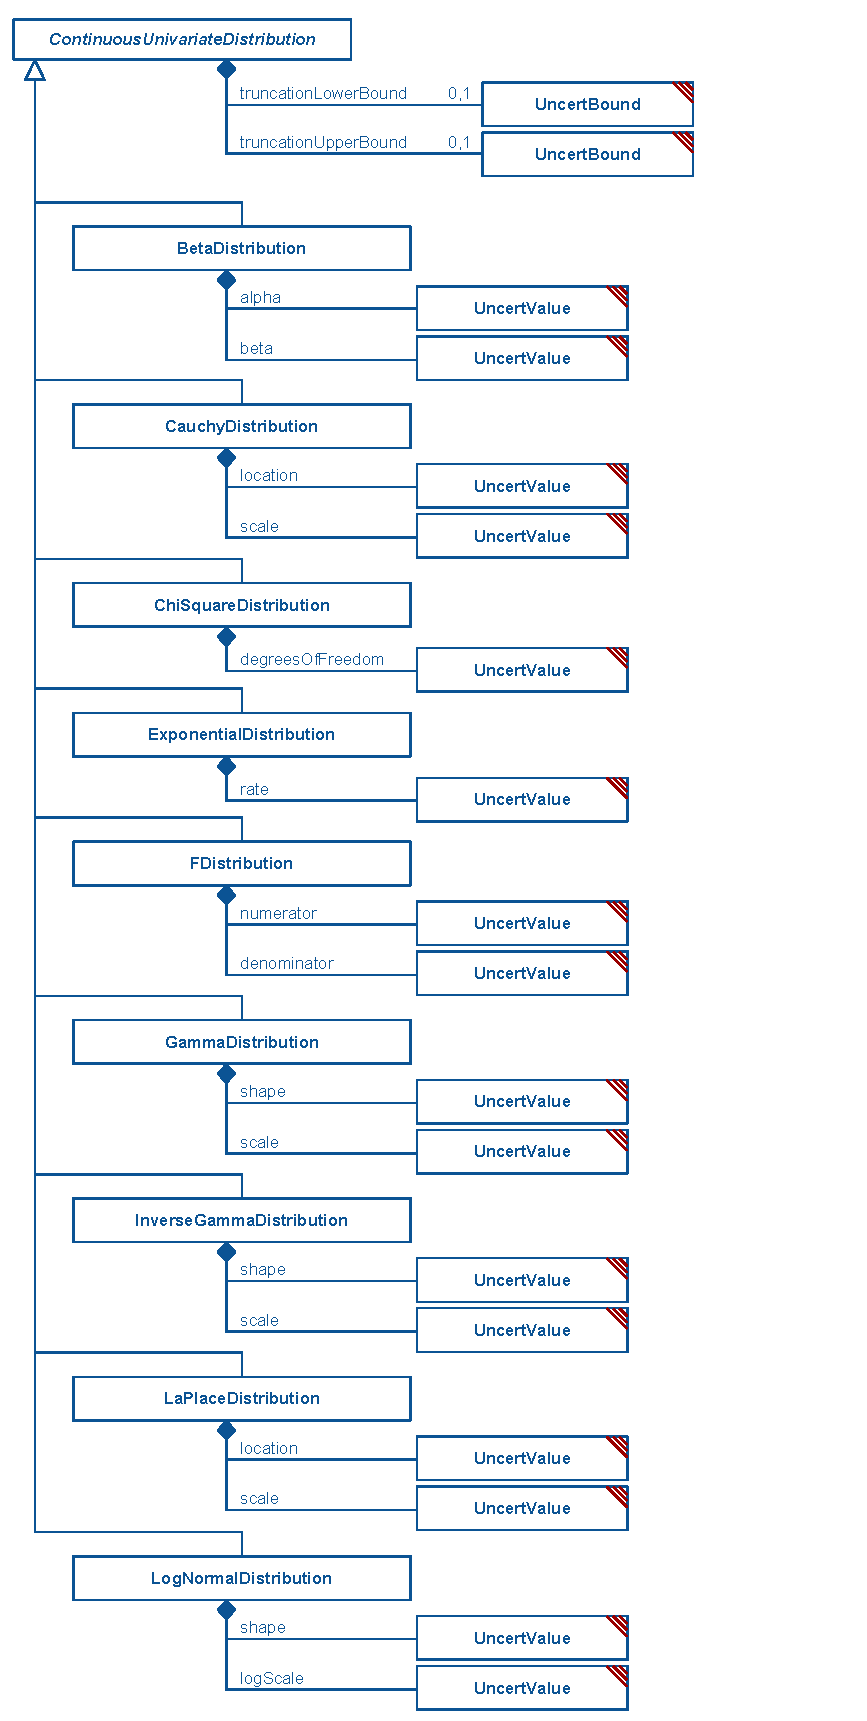
\includegraphics[width=0.6\linewidth]{figs/continuousUnivariateDistribution_first.pdf}
\caption{The definition of the \ContinuousUnivariateDistribution abstract class, and its \BetaDistribution, \CauchyDistribution, \ChiSquareDistribution, \ExponentialDistribution, \FDistribution, \GammaDistribution, \InverseGammaDistribution, \LaplaceDistribution, and \LogNormalDistribution children.  All may have lower and upper \UncertBound children, and each has one or more other parameters encoded as \UncertValue children (both defined below).}
\label{fig:continuousUnivariateDistribution_first}
\end{figure}


\subsection{The \class{ContinuousUnivariateDistribution} class}
\label{ContinuousUnivariateDistribution-class}
\label{continuousunivariatedistribution-class}
The abstract \ContinuousUnivariateDistribution class is the base class for a wide variety of distributions, all of which describe a potentially-bounded continuous range of probabilities.  Many of the most commonly-used distributions such as the \NormalDistribution and the \UniformDistribution fall into this category.

\begin{figure}[htb]
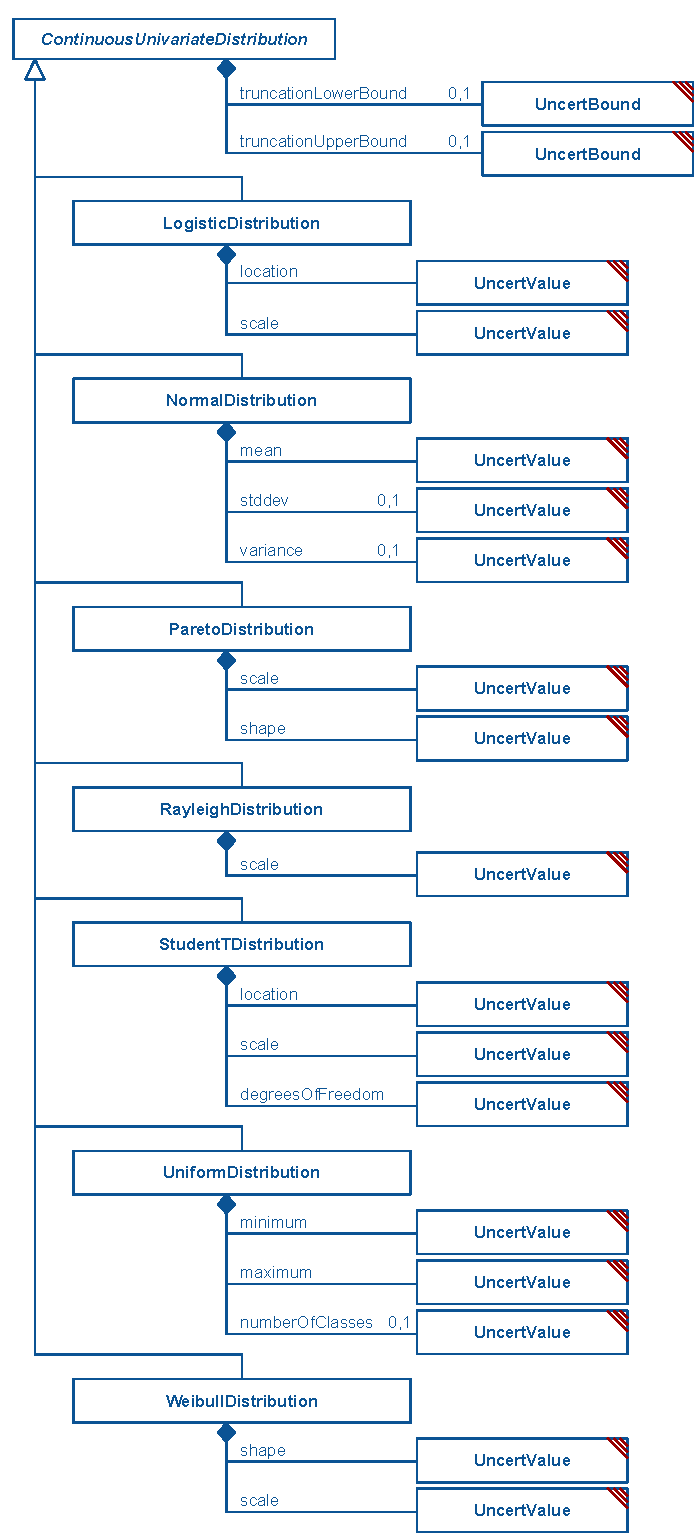
\includegraphics[width=0.55\linewidth]{figs/continuousUnivariateDistribution_second.pdf}
\caption{The definition of the \ContinuousUnivariateDistribution abstract class, and its \LogisticDistribution, \NormalDistribution, \ParetoDistribution, \RayleighDistribution, \StudentTDistribution, \UniformDistribution, and \WeibullDistribution children.  All may have lower and upper \UncertBound children, and each has one or more other parameters encoded as \UncertValue children (both defined below).}
\label{fig:continuousUnivariateDistribution_second}
\end{figure}

All \ContinuousUnivariateDistribution elements may have two optional children: \val{lowerTruncationBound} and \val{upperTruncationBound}, both of the class \UncertBound (defined below).  Either element, if present, limit the range of possible sampled values from the distribution.  The \val{lowerTruncationBound} defines the lowest value (inclusive or not, as defined by that element's \token{inclusive} attribute) that can be sampled, and the \val{upperTruncationBound} defines the highest.  If both children are present, the \val{lowerTruncationBound} must either be lower than the \val{upperTruncationBound}, or they may be equal, if both bounds are set \token{inclusive}=\val{true}.  Similarly, some distributions are themselves naturally bound (some may, for example, only return values greater than zero).  In those cases, the natural lower bound of the distribution must either be lower than the \val{upperTruncationBound}, or be equal to it if the natural lower bound is inclusive, and if the \val{upperTruncationBound} is set \token{inclusive}=\val{true}.  Similarly, the natural upper bound of the distribution must either be higher than the \val{lowerTruncationBound}, or it may be equal to it if the natural upper bound is inclusive and if the \val{lowerTruncationBound} is set \token{inclusive}=\val{true}.  It may be impossible to determine this from a static analysis of the model, as either or both bound's values may depend on other dynamic variables.  If a simulator encounters this situation, the sampled value and the behavior of the simulator are undefined.

If bounded, the cumulative probability that would have been assigned to the region outside the bound is re-assigned proportionally to the rest of the distribution.  It should be noted that while discarding any value obtained from the non-truncated version of the distribution and re-sampling is indeed one method that could be used to accomplish this, the efficiency of that algorithm decreases with the width of the allowed window, and indeed is technically zero (and would take an infinite amount of time to complete) should the bounds be equal to one another.  Taking any samples obtained outside the bound window and instead returning the boundary value itself is incorrect, and will not result in a proper draw from the defined distribution.

The distributions of this type allowed in this version of the specification are defined in \fig{fig:continuousUnivariateDistribution_first} and \fig{fig:continuousUnivariateDistribution_second}.  A full list of all of the distributions is provided in \sec{sec:allDistributions}.


\begin{figure}[htb]
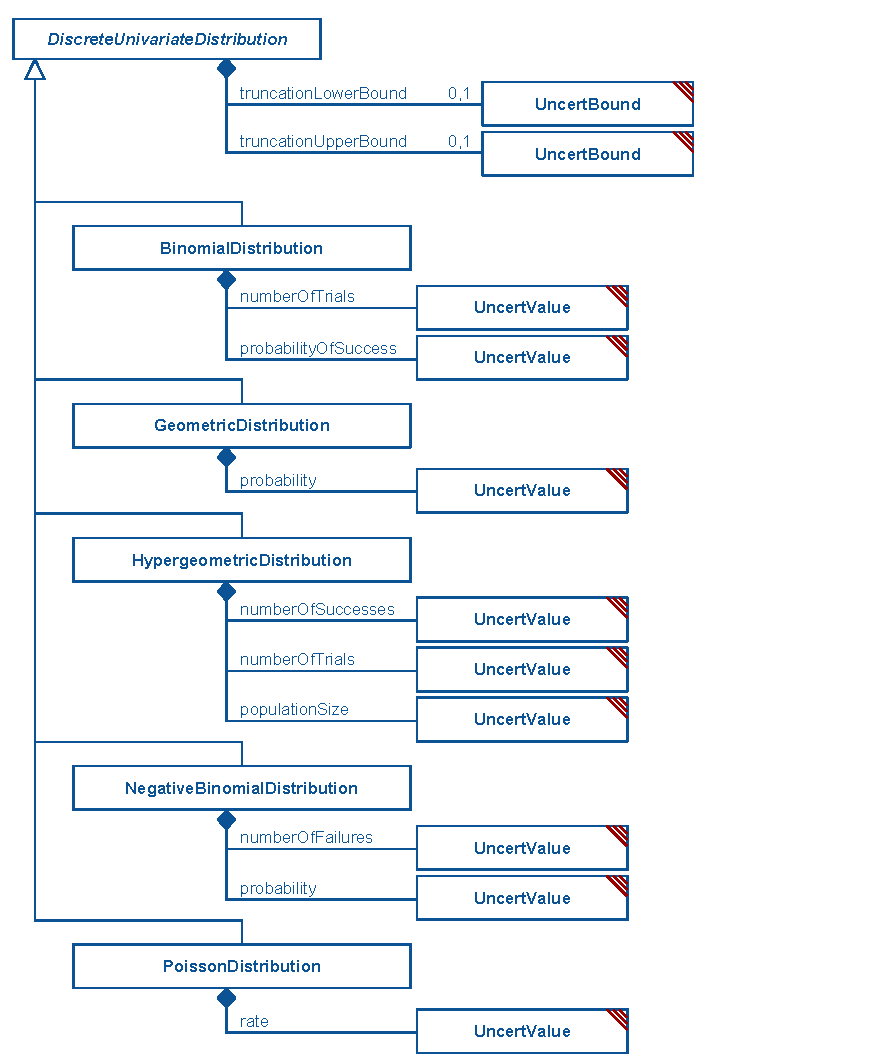
\includegraphics[width=0.7\linewidth]{figs/discreteUnivariateDistribution.pdf}
\caption{The definition of the \DiscreteUnivariateDistribution abstract class, and its \BinomialDistribution, \GeometricDistribution, \HypergeometricDistribution, \NegativeBinomialDistribution, and \PoissonDistribution children.  All may have lower and upper \UncertBound children, and each has one or more other parameters encoded as \UncertValue children (both defined below).}
\label{fig:discreteUnivariateDistribution}
\end{figure}

\subsection{The \class{DiscreteUnivariateDistribution} class}
\label{DiscreteUnivariateDistribution-class}
\label{discreteunivariatedistribution-class}

The abstract \DiscreteUnivariateDistribution class is the base class for a wide variety of distributions, all of which describe a potentially-bounded range of probabilities of discrete values.  The most commonly-used distributions in this class is probably the \PoissonDistribution.  Distributions that always return integers fall in this category, which often involve events happening at particular frequencies.

All \DiscreteUnivariateDistribution elements (like \ContinuousUnivariateDistribution elements) may have two optional children: \val{lowerTruncationBound} and \val{upperTruncationBound}, both of the class \UncertBound (defined below).  Either element, if present, limit the range of possible sampled values from the distribution.  The \val{lowerTruncationBound} defines the value below which no sampling may take place
(inclusive or not, as defined by that element's \token{inclusive} attribute), and the \val{upperTruncationBound} defines the value above which no sampling may take place.  These bounds may fall between the possible discrete values being returned:  as an example, for a distribution that returned an integer in the series [0, 1, 2, ...], if it was given a \val{lowerTruncationBound} of 1.5, the lowest value it could return would be 2.  In this case, the value of the \token{inclusive} attribute on the \UncertBound would be immaterial, as '1.5' could never be returned.

As \changed{with} \ContinuousUnivariateDistribution bounds, if both bounds are present, the \val{lowerTruncationBound} must either be lower than the \val{upperTruncationBound}, or they may be equal, if both bounds are set \token{inclusive}=\val{true}.  Similarly, the discrete distributions are themselves often naturally bound (some may, for example, only return values greater than zero).  In those cases, the natural lower bound of the distribution must be either be lower than the \val{upperTruncationBound}, or it may be equal to it if the natural lower bound is inclusive, and if the \val{upperTruncationBound} is set \token{inclusive}=\val{true}.  Similarly, the natural upper bound of the distribution must either be higher than the \val{lowerTruncationBound}, or it may be equal to it if the natural upper bound is inclusive and if the \val{lowerTruncationBound} is set \token{inclusive}=\val{true}.  In addition, if both bounds are defined, they must define a span within which at least one possible sampled discrete value may be found.  For a distribution that returns integers, for example, one may not define a lower bound of 1.5 and an upper bound of 1.8, as no integer lies within that range.  It may be impossible to determine if any of these rules are violated from a static analysis of the model, as either or both bound's values may depend on other dynamic variables.  If a simulator encounters this situation, the sampled value and the behavior of the simulator are undefined.

If bounded, the cumulative probability that would have been assigned to the values outside the bound is re-assigned proportionally to the rest of the distribution.  It should be noted that while discarding any value obtained from the non-truncated version of the distribution and re-sampling is indeed one method that could be used to accomplish this, the efficiency of that algorithm decreases with the width of the allowed window, and indeed is technically zero (and could take an infinite amount of time to complete) should the bounds allow only a single discrete value.  Taking any samples obtained outside the bound window and instead returning the boundary value itself is incorrect, and will not result in a proper draw from the defined distribution.

The distributions of this type allowed in this version of the specification are defined in \fig{fig:discreteUnivariateDistribution}.  A full list of all of the distributions is provided in \sec{sec:allDistributions}.



\begin{figure}[htb]
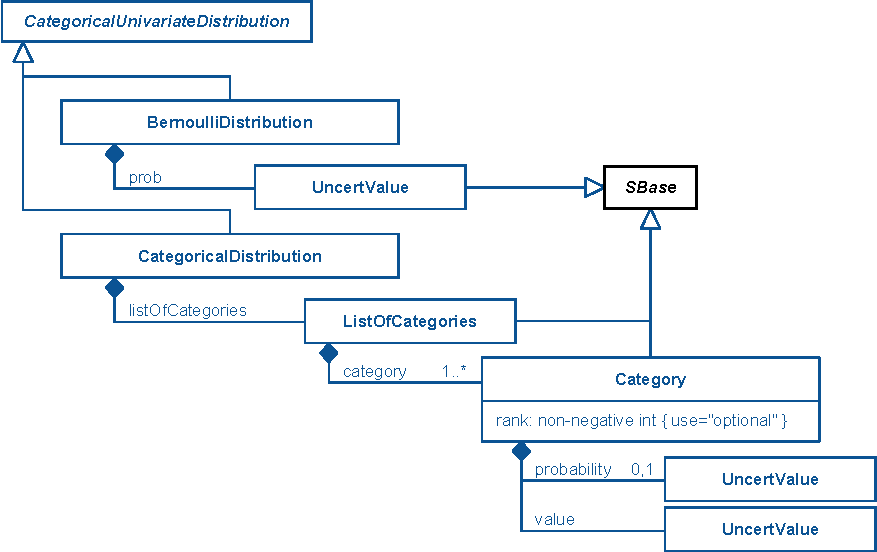
\includegraphics[width=0.8\linewidth]{figs/categoricalUnivariateDistribution.pdf}
\caption{The definition of the \CategoricalUnivariateDistribution abstract class, plus the \BernoulliDistribution, \CategoricalDistribution, \ListOfCategories, and \Category classes.}
\label{fig:categoricalUnivariateDistribution}
\end{figure}

\subsection{The \class{CategoricalUnivariateDistribution} class}
\label{CategoricalUnivariateDistribution-class}
\label{categoricalunivariatedistribution-class}

The \CategoricalUnivariateDistribution abstract class includes distributions where the various possible sampled values are each explicitly listed, along with the probability for that sampled value.  The sum of these probabilities must therefore equal 1.0, in order to be valid.  This type of distribution class is used for things such as weighted die rolls, or other situations where particular values are obtained at arbitrary probabilities.

Because each possible sampled value is explicitly listed in an \CategoricalUnivariateDistribution, it does not have the optional \UncertBound values that the other univariate distributions do: if a particular value is not allowed, it is simply dropped from the list of options, and the probabilities of the other values are scaled accordingly.


\begin{figure}[htb]
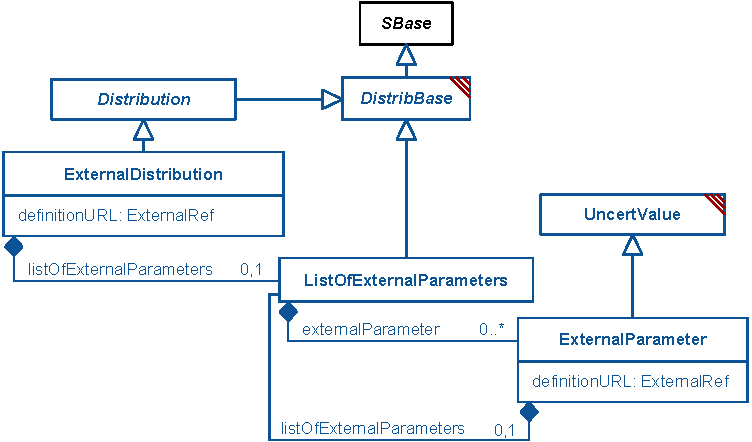
\includegraphics[width=0.5\linewidth]{figs/externalDistribution.pdf}
\caption{The definition of the \ExternalDistribution, \ExternalParameter, and \ListOfExternalParameters classes.  These classes define a way to define a distribution with reference to an external database or ontology of distribution definitions.}
\label{fig:externalDistribution}
\end{figure}

\subsection{The \class{ExternalDistribution} class}
\label{ExternalDistribution-class}
\label{externaldistribution-class}

The \ExternalDistribution class is provided to allow a modeler to encode a distribution not otherwise explicitly handled by this specification.  Because the range of possibilities is so vast, the modeler should not normally expect any given SBML simulator or other software to be able to properly manipulate this distribution, but particular software tools may implement support for certain distributions they know their own software's users may require.

The required attribute \token{definitionURL}, of type \primtype{ExternalRef}, must be a URI that defines a valid distribution.  It is strongly recommended that modelers use distributions from ProbOnto (\url{http://probonto.org/}), as consistently referencing a single ontology will improve exchangeability, at least slightly.  The referenced distribution is then the distribution defined by this \ExternalDistribution, along with any parameterization provided by the children \ExternalParameter elements.

Some referenced distributions are multivarite, meaning they define correlated distributions for two or more parameters.  It is impossible with \sbmlthreecore to define a \FunctionDefinition that returns a vector, and similarly no \primtype{SId} in \sbmlthreecore can be used to represent a vector.  If this is desired, then, the Arrays package must be used in concert with the \ExternalDistribution to cooperatively set up a model with a \FunctionDefinition that can use an array as input and/or as output.

The \ExternalDistribution defines an optional child \ListOfExternalParameters, which can be used to parameterize the defined distribution.


\subsection{Specific Distributions}
\label{sec:allDistributions}

In this table, all distributions are listed, along with their types (Continuous, Categorical, or Discrete), whether they're univariate or multivariate, and a brief description.  The element name is the name of the distribution with spaces removed, the initial letter lower-cased, and \val{Distribution} appended, so, for example, the \val{Exponential} distribution becomes \val{<exponentialDistribution>}, and the \val{Student T} distribution becomes \val{<studentTDistribution>}.
%The exception is that all of the mixture models (ones that end with \val{Mixture Model}), only have spaces removed but nothing appended:  the Continuous Univariate Mixture Model becomes \val{<ContinuousUnivariateMixtureModel>}, etc.

All of these distributions inherit from the abstract \Distribution class.  Additionally, the appropriate distributions inherit from the \UnivariateDistribution or \MultivariateDistribution abstract classes, and further from the \ContinuousUnivariateDistribution, \DiscreteUnivariateDistribution, or \CategoricalUnivariateDistribution classes, which are related to one another as one would expect.

All descriptions are based on the information from \url{http://www.uncertml.org/}, which is now defunct, but which can still be accessed at \url{http://web.archive.org/web/20160313012501/uncertml.org}.

Distributions are listed grouped by category (type and univarite/multivariate), and alphabetical within those categories.


\subsection{The \class{BetaDistribution} class}
\label{BetaDistribution-class}
\label{betadistribution-class}

The \BetaDistribution is a \ContinuousUnivariateDistribution that defines the \UncertValue children \token{alpha} ($\alpha$) and \token{beta} ($\beta$).  Both \token{alpha} and \token{beta} must be positive.

A random variable x is Beta distributed if the probability density function (pdf) is of the form:

\begin{center}
$\dfrac{1}{B\left(\alpha,\beta\right)}x^{\alpha-1}\left(1-x\right)^{\beta-1}$, where $B\left(\alpha,\beta\right)$ = $\dfrac{\Gamma\left(\alpha\right)\Gamma\left(\beta\right)}{\Gamma\left(\alpha+\beta\right)}$
\end{center}

The distribution is usually denoted as $x\sim Be\left(\alpha,\beta\right)$ with parameters $\alpha$ and $\beta$, both positive real values. As the domain of the random variable is defined to be $[0,1]$ the Beta distribution is normally used to describe the distribution of a probability value.

\subsection{The \class{CauchyDistribution} class}
\label{CauchyDistribution-class}
\label{cauchydistribution-class}

The \CauchyDistribution is a \ContinuousUnivariateDistribution that defines the \UncertValue children \token{location} ($\theta$) and \token{scale} ($\gamma$).  The \token{scale} value must be positive.

A random variable x follows a Cauchy distribution if the probability density function (pdf) is of the form:

\begin{center}
$\dfrac{1}{\pi\gamma}\left[1+\left(\dfrac{x-\theta}{\gamma}\right)^2\right]^{-1}$
\end{center}

The Cauchy distribution is equivalent to a Student-T distribution with 1 degree of freedom. It is widely used in physics, optics and astronomy. It is also known as the Lorenz or the Breit-Wigner distribution.

\subsection{The \class{ChiSquareDistribution} class}
\label{ChiSquareDistribution-class}
\label{chisquaredistribution-class}

The \ChiSquareDistribution is a \ContinuousUnivariateDistribution defining a \UncertValue child \token{degreesOfFreedom} ($\nu$).  The \token{degreesOfFreedom} must be a positive integer.

A random variable x is Chi-square distributed if the probability density function (pdf) is of the form:

\begin{center}
$\dfrac{1}{\Gamma(\nu/2)2^{\nu/2}}x^{\nu/2-1}exp(-x/2)$
\end{center}

The distribution is usually denoted as $x\sim\chi_\nu$ where $\nu$ is known as the degrees of freedom parameter. $\nu$ has to be positive and $x$ has to be non-negative for the density to be defined. The Chi-square distribution is a special case of the Gamma distribution where $\chi \sim\Gamma(k=\nu/2,\theta=2)$.

\subsection{The \class{ExponentialDistribution} class}
\label{ExponentialDistribution-class}
\label{exponentialdistribution-class}

The \ExponentialDistribution is a \ContinuousUnivariateDistribution that defines the \UncertValue child \token{rate} ($\lambda$).  The \token{rate} value must be positive.

A random variable x follows an exponential distribution if the probability density function (pdf) is of the form:

\begin{center}
$\lambda e^{-\lambda x}$
\end{center}

It is often represented as $x \sim$ Exp$(\lambda)$. It is used to model the time between events for a Poisson process and is used in simulation of stochastic systems.

\subsection{The \class{FDistribution} class}
\label{FDistribution-class}
\label{fdistribution-class}

The \FDistribution is a \ContinuousUnivariateDistribution that defines the \UncertValue children \token{numerator} ($\nu_1$) and \token{denominator} ($\nu_2$).  Both \token{numerator} and \token{denominator} must be positive integers.

A random variable x follows an F distribution if the probability density function (pdf) is of the form:

\begin{center}
$\dfrac{ 1 } {B(\nu_1/2, \nu_2/2)} \left( \dfrac{\nu_1}{\nu_2}\right)^{\nu_1/2} x^{\nu_1/2 - 1} \left(1 + \dfrac{\nu_1}{\nu_2}x \right)^{-\frac{\nu_1+\nu_2}{2} }$
\end{center}

where $B(.)$ is the Beta function. It often arises as the ratio of two random variables that are identically Chi-Square distributed.

\subsection{The \class{GammaDistribution} class}
\label{GammaDistribution-class}
\label{gammadistribution-class}

The \GammaDistribution is a \ContinuousUnivariateDistribution that defines the \UncertValue children \token{shape} ($k$) and \token{scale} ($\theta$).  Both \token{shape} and \token{scale} must be positive.

A random variable x is Gamma distributed if the probability density function (pdf) is of the form:

\begin{center}
$\dfrac{1}{\Gamma(k) \theta^k} x^{k-1} exp(-x/\theta) $ with $ \Gamma(\cdot) $ the Gamma function.
\end{center}

The distribution is usually denoted as $x \sim Gamma(k, \theta)$ where $k$ is known as the shape parameter and $\theta$ the scale parameter. Both parameters have be positive and $x$ has to be non-negative for the density to be defined. In practice the Gamma distribution is often use to model the distribution of non-negative quantities such as variances.

\subsection{The \class{InverseGammaDistribution} class}
\label{InverseGammaDistribution-class}
\label{inversegammadistribution-class}

The \InverseGammaDistribution is a \ContinuousUnivariateDistribution that defines the \UncertValue children \token{shape} ($\alpha$) and \token{scale} ($\beta$).  Both \token{alpha} and \token{beta} must be positive.

A random variable x is Inverse Gamma distributed if the probability density function (pdf) is of the form:

\begin{center}
$\dfrac{\beta^\alpha}{\Gamma(\alpha)}x^{-\alpha-1}exp(-\beta/x)$
\end{center}

If variable $x$ is Inverse Gamma distributed, 1/$x$ is gamma distributed. The Inverse Gamma distribution function can be obtained from the Gamma distribution by a transformation of variables.

\subsection{The \class{LaplaceDistribution} class}
\label{LaplaceDistribution-class}
\label{laplacedistribution-class}

The \LaplaceDistribution is a \ContinuousUnivariateDistribution that defines the \UncertValue children \token{location} ($\mu$) and \token{scale} ($b$).  The \token{scale} value must be positive.

A random variable x is Laplace distributed if the probability density function (pdf) is of the form:

\begin{center}
$\dfrac{1}{2b}\mathrm{exp}\bigg(-\dfrac{abs(x-\mu)}{b}\bigg)$
\end{center}

where $abs$ denotes the absolute value. It can be thought of as a combination of two exponential distributions.

\subsection{The \class{LogNormalDistribution} class}
\label{LogNormalDistribution-class}
\label{lognormaldistribution-class}

The \LogNormalDistribution is a \ContinuousUnivariateDistribution that defines the \UncertValue children \token{shape} ($\sigma^2$) and \token{logScale} ($\mu$).  The \token{shape} value must be positive.

A random variable x is Log Normal distributed if the probability density function (pdf) is of the form:

\begin{center}
$\dfrac{1}{x \sqrt{2 \pi \sigma^2}} \mathrm{exp}\bigg(-\dfrac{ (\mathrm{ln}(x)-\mu)^2 }{2 \sigma^2}\bigg)$
\end{center}

If variable x is normally distributed, exp(x) is Log Normal distributed. The Log Normal distribution function can be obtained from the normal distribution by a transformation of variables. It is often used for variables that must be positive.

\subsection{The \class{LogisticDistribution} class}
\label{LogisticDistribution-class}
\label{logisticdistribution-class}

The \LogisticDistribution is a \ContinuousUnivariateDistribution that defines the \UncertValue children \token{location} ($\mu$) and \token{scale} ($s$).  The \token{scale} value must be positive.

A random variable x is Logistic distributed if the probability density function (pdf) is of the form:

\begin{center}
$\dfrac{\mathrm{exp}(-(x-\mu)/s)}{s(1+\mathrm{exp}\big(-(x-\mu)/s)\big)^2}$
\end{center}

\subsection{The \class{NormalDistribution} class}
\label{NormalDistribution-class}
\label{normaldistribution-class}

The \NormalDistribution is a \ContinuousUnivariateDistribution that defines the \UncertValue children \token{mean} ($\mu$), \token{stddev} ($\sigma$), and \token{variance} ($\sigma^2$).  The distribution must either define a \token{stddev} or a \token{variance}, but not both.  The \token{variance}, if defined, must be positive.

A random variable x is normally distributed if the probability density function (pdf) is of the form:

\begin{center}
$\dfrac{1}{\sqrt{2\pi\sigma^2}}\mathrm{exp}\big(-\frac{(x-\mu)^2}{2\sigma^2}\big)$
\end{center}

The distribution is usually denoted as $x\sim \mathcal{N}(\mu,\sigma^2)$ where $\mu$ is known as the mean parameter and $\sigma^2$ the variance parameter. If the random variable x is a vector of length greater than one, the normal distribution can be generalised to the Multivariate normal.  A reason for the widespread usage of the normal distribution is the Central limit theorem which states that the distribution of the mean of a large number of independent identically distributed random variables tends to a normal distributions as the number of random variables increases.

\subsection{The \class{ParetoDistribution} class}
\label{ParetoDistribution-class}
\label{paretodistribution-class}

The \ParetoDistribution is a \ContinuousUnivariateDistribution that defines the \UncertValue children \token{scale} ($x_m$) and \token{shape} ($\alpha$).  Both \token{shape} and \token{scale} must be positive.

A random variable x follows a Pareto distribution if the probability density function is of the form:

\begin{center}
$\dfrac{\alpha x_m^\alpha}{x^{\alpha+1}}$
\end{center}

The distribution allows for the specification of a minimum value below which the density is 0. It is a skewed heavy-tailed distribution.

\subsection{The \class{RayleighDistribution} class}
\label{RayleighDistribution-class}
\label{rayleighdistribution-class}

The \RayleighDistribution is a \ContinuousUnivariateDistribution that defines the \UncertValue children \token{scale}.

[From Wikipedia:] A Rayleigh distribution is often observed when the overall magnitude of a vector is related to its directional components. One example where the Rayleigh distribution naturally arises is when wind velocity is analyzed into its orthogonal 2-dimensional vector components. Assuming that each component is uncorrelated, normally distributed with equal variance, and zero mean, then the overall wind speed (vector magnitude) will be characterized by a Rayleigh distribution. A second example of the distribution arises in the case of random complex numbers whose real and imaginary components are independently and identically distributed Gaussian with equal variance and zero mean. In that case, the absolute value of the complex number is Rayleigh-distributed.

\subsection{The \class{StudentTDistribution} class}
\label{StudentTDistribution-class}
\label{studenttdistribution-class}

The \StudentTDistribution is a \ContinuousUnivariateDistribution that defines the \UncertValue children  \token{location} ($\mu$), \token{scale} ($\sigma^2$) and \token{degreesOfFreedom} ($\nu$).

A random variable x follows a Student-t distribution if the probability density function (pdf) is of the form:

\begin{center}
$\dfrac{\Gamma(\nu/2+1/2)}{\Gamma(\nu/2)(\pi\nu\sigma^2)^{1/2}}\big[1+\frac{(x-\mu)^2}{\nu\sigma^2}\big]^{-\nu/2-1/2}$. The distribution is usually denoted as $x\sim St(\mu,\lambda,\nu)$
\end{center}

This distribution corresponds to integrating out the variance of a normal distribution using a inverse Gamma prior. It can therefore be interpreted as an infinite mixture of normal distributions having the same mean but different variances. The three parameters are the mean ($\mu$), degrees of freedom ($\nu$) and variance ($\sigma^2$). Setting the variance to 1 and the mean to 0 we obtain the Student-t form found in standard statistics references such as Wikipedia. Setting the d.f. to 1 the Cauchy distribution is obtained. Setting the d.f. to infinity the normal distribution is obtained. The student-t distribution is commonly used in likelihood inference as the maximum likelihood parameter estimates are more robust to outlier observations compared to the normal distribution.

\subsection{The \class{UniformDistribution} class}
\label{UniformDistribution-class}
\label{uniformdistribution-class}

The \UniformDistribution is a \ContinuousUnivariateDistribution that defines the \UncertValue children \token{minimum} ($a$), \token{maximum} ($b$) and the optional \token{numberOfClasses}.  The \token{minimum} value must be less than the \token{maximum} value.  If \token{numberOfClasses} is defined, its value must be an integer greater than or equal to two.

A random variable x follows a uniform distribution if the probability density function (pdf) is of the form:

\begin{center}
$\dfrac{1}{b-a}$
\end{center}

The distribution assigns equal probability to all events within the chosen domain between (and including) the minimum ($a$) and the maximum ($b$).

If \token{numberOfClasses} is included, the uniform range is divided into $numberOfClasses-1$ sections, and each of the borders of those sections are equally likely to be returned.  If \token{numberOfClasses} is 2 (the minimum), the range just has $2-1=1$ section, and the borders of that section (the \token{minimum} and \token{maximum}) are the two possible return values.  If \token{numberofClasses} is 3, the range is broken into $3-1=2$ sections, leaving the \token{minimum}, \token{maximum}, and mean as the three possible return values, etc.

\subsection{The \class{WeibullDistribution} class}
\label{WeibullDistribution-class}
\label{weibulldistribution-class}

The \WeibullDistribution is a \ContinuousUnivariateDistribution that defines the \UncertValue children \token{shape} ($k$) and \token{scale} ($\lambda$).  Both \token{shape} and \token{scale} must be positive.

A random variable x follows an Weibull distribution if the probability density function (pdf) is of the form:

\begin{center}
$\dfrac{k}{\lambda}\left(\dfrac{x}{\lambda}\right)^{k-1}\mathrm{exp}\bigg(\dfrac{-x}{\lambda}\bigg)^k$
\end{center}

It includes the exponential distribution as a special case. It is often used in engineering and finance.

%Continuous Multivariate Mixture Model & Continuous & Multivariate 
%  & A mixture model is a linear combination of base distributions. A widely used case is where the base distributions are Gaussian in which case the model is known as the Gaussian Mixture Model.
%Dirichlet & Continuous & Multivariate 
%  & A $K$ dimensional random variable x follows a Dirichlet distribution if the probability density function (pdf) is of the form $\frac{1}{B(\mathbf{a})} \prod_{i=1}^K x_i^{\alpha_i - 1}$ where $B(\mathbf{a}) = \frac{ \prod^k_{i=1} \Gamma(\alpha_i) } { \Gamma( \sum_{i=1}^K \alpha_i ) }$ and $\Gamma(.)$ is the Gamma function. It is the multivariate extension of the beta distribution to higher dimensions with K a positive integer greater than or equal to 2.
%Multivariate Normal & Continuous & Multivariate 
%  & The Multivariate Normal is an extension of the univariate normal distribution to higher dimensional vector spaces. A random vector variable of dimension $ k $  denoted $ \mathbf{x} $ is normally distributed if the probability density function (pdf) is of the form $(2 \pi)^{-k/2} \mathrm{det}(\Sigma)^{-1/2} exp (-\frac{1}{2} (\mathbf{x} - \mathbf{\mu})^T \Sigma^{-1} (\mathbf{x} - \mathbf{\mu}) ) $ where $ \mathrm{det}(.) $ denotes the determinant and $ (.)^T $ the matrix transpose. The distribution is usually denoted as $ \mathbf{x} \sim \mathcal{N}(\mathbf{\mu}, \Sigma) $ where $ \mathbf{\mu} $ is known as the mean vector parameter and $ \Sigma $ the covariance matrix parameter.
%Multivariate Student T & Continuous & Multivariate 
%  & A random variable $ \mathbf{x} $ follows a multivariate Student-t distribution if the probability density function (pdf) is of the form $\frac{ \Gamma(\nu/2 + k/2)} {\Gamma(\nu/2) (\pi \nu)^{k/2} \mathrm{det} (\Sigma)^{1/2} } \left[1 + \frac{ \Delta^2 } { \nu } \right]^{-\nu/2 - k/2}  $ where $ \Delta^2 = (\mathbf{x} - \mathbf{\mu})^T \Sigma^{-1}  (\mathbf{x} - \mathbf{\mu}) $ is the squared Mahalanobis distance. The distribution is usually denoted as $ x \sim St(\mathbf{\mu},\Sigma,\nu) $. It is the extension of the univariate student-t distribution to higher dimensions. Student-t distributions are often used when tails are expected to be heavier than Gaussian or Normal, and can result from applying Bayesian inference.
%Normal Inverse Gamma & Continuous & Multivariate 
%  & A Normal Inverse Gamma distribution is the conjugate prior of a normal distribution with unknown mean and variance. It is the coupled product of an Inverse Gamma distribution and a normal distribution. In particular if $p(\mathbf{X} ; \mu, \sigma^2) $ is the likelihood function of a Normally distributed set of random variables with mean $ \mu $ and variance $ \sigma^2 $ and if both the mean and variance are considered unknown, the conjugate prior is $  p(\mu,\sigma^2) = p(\mu ; \sigma^2) p(\sigma^2) $ where $  p(\mu ; \sigma^2) = \mathcal{N}(\mu ; \mu_0, \sigma^2/\nu) $ a Normal prior on the mean and $ p(\sigma^2) = \mathrm{IG}(\sigma^2 ; \alpha, \beta) $ an Inverse Gamma prior on the variance. Note that the priors are not independent as the prior variance of the mean is a linear function of of the variance $ \sigma^2 $. It is also common to use a Normal-Gamma distribution where a conjugate prior is placed on the unknown mean and precision (i.e. inverse variance) of the Normal likelihood in which case the prior is a product of a Normal and Gamma distributions. In the case of a Multivariate normal likelihood, the corresponding conjugate prior is a Normal-Wishart distribution.

\subsection{The \class{BinomialDistribution} class}
\label{BinomialDistribution-class}
\label{binomialdistribution-class}

The \BinomialDistribution is a \DiscreteUnivariateDistribution that defines the \UncertValue children \token{numberOfTrials} ($n$) and \token{probabilityOfSuccess} ($\theta$).  The \token{numberOfTrials} must be a positive integer, and \token{probabilityOfSuccess} must be a value between zero and one, inclusive.

A random variable $ x $ follows a Binomial distribution if the probability mass function (pmf) is of the form:

\begin{center}
${n \choose x} \theta^x (1-\theta)^{n-x} $
\end{center}

where $ {n \choose x} $ denotes $ n $ choose $ x $. The distribution is usually denoted as $ x \sim b(n,\theta) $. The distribution describes the probability of getting $ x $ successes in $n$ trials of independent experiments that have the same probability of success.

\subsection{The \class{GeometricDistribution} class}
\label{GeometricDistribution-class}
\label{geometricdistribution-class}

The \GeometricDistribution is a \DiscreteUnivariateDistribution that defines the \UncertValue child \token{probability} ($p$).  The \token{probability} must have a value must be between zero and one, inclusive.

A random variable $ x $ follows a geometric distribution if the probability mass function (pmf) is of the form:

\begin{center}
$(1-p)^{x-1} p$
\end{center}

It is often represented as $x \sim \mathrm{Geom}(p)$. It is the discrete analogue of the exponential distribution. It is used to model distribution of the number of binary (Bernoulli) trials needed to get one success, with parameter, probability $p$.

\subsection{The \class{HypergeometricDistribution} class}
\label{HypergeometricDistribution-class}
\label{hypergeometricdistribution-class}

The \HypergeometricDistribution is a \DiscreteUnivariateDistribution that defines the \UncertValue children \token{numberOfSuccesses} ($m$). \token{numberOfTrials} ($n$), and \token{populationSize} ($N$).  All three values must be positive integers, chosen such that \token{numberOfTrials} is less than or equal to \token{populationSize}.

A random variable $ x $ follows a hypergeometric distribution if the probability mass function (pmf) is of the form:

\begin{center}
$\dfrac{ {m \choose k} { N-m \choose n-k } } { {N \choose n}}$
\end{center}

probability of getting $x$ successes.  It describes the number of successes in a sequence of draws without replacement.

\subsection{The \class{NegativeBinomialDistribution} class}
\label{NegativeBinomialDistribution-class}
\label{negativebinomialdistribution-class}

The \NegativeBinomialDistribution is a \DiscreteUnivariateDistribution.  It has two defined \UncertValue children \token{numberOfFailures} ($r$) and \token{probability} ($p$). The \token{numberOfFailures} must be a positive integer, and \token{probability} must have a value between zero and one, inclusive.

A random variable $ x $ follows a Negative Binomial distribution if the probability mass function (pmf) is of the form:

\begin{center}
${x + r - 1 \choose x} p^x (1-p)^r $
\end{center}

The distribution describes the probability of getting $ x $ successes in trials of independent experiments that have the same probability of success, and are run until we observe $ r $ failures.  Note that some systems formulate this distribution differently:  observing $k$ failures before obtaining the $r^{th}$ success.  The formulation above follows the English version of Wikipedia; the alternate formulation is used on other language Wikipedia definitions of the distribution, as well as various software packages like Matlab and R.

{\color{red} Lucian: \controversial NOTE!  The above formulation was used by UncertML and Wikipedia, the sort-of-default distribution definition source for the annotation scheme.  However, once people actually start implementing it, they may find that their software package uses the alternative.  The ProbOnto 2.5 specification (\url{https://sites.google.com/site/probonto/download}) goes into great detail on this issue in Appendix A.3, for anyone who wants to know more.  I would be happy to change the definition to match people's software, if need be.}


\subsection{The \class{PoissonDistribution} class}
\label{PoissonDistribution-class}
\label{poissondistribution-class}

The \PoissonDistribution is a \DiscreteUnivariateDistribution that defines the \UncertValue child \token{rate} ($\lambda$).  The \token{rate} value must be positive.

A random variable $ x $ follows a Poisson distribution if the probability mass function (pmf) is of the form:

\begin{center}
$\dfrac{\lambda^x}{x!} \mathrm{exp}(-\lambda)$
\end{center}

The Poisson distribution can be used to model the number of events occurring within fixed time period of time.


%Discrete Multivariate Mixture Model & Discrete & Multivariate 
%  & A mixture model is a linear combination of base distributions. A widely used case is where the base distributions are Gaussian in which case the model is known as the Gaussian Mixture Model.
%Multinomial & Discrete & Multivariate 
%  & A random variable $ x $ follows a Multinomial distribution if the probability mass function (pmf) is of the form $\frac{N!}{x_1! \dots x_k!} \prod_{i=1}^K p_i^{x_i}$. The Multinomial distribution is a multivariate generalisation of the Binomial distribution for a $ K $ state variable to be in state $ k $ given $N$ observations. This can be confused with the Categorical distribution (added at version 3.0 of UncertML) which can be considered a Multinomial distribution when a 1 of K encoding is used.
%Wishart & Discrete & Multivariate 
%  & A random matrix variable $ \mathbf{X} $ of size $ D \times D $ follows a Wishart distribution if the probability density function is of the form $\mathrm{det}(\mathbf{W})^{-\nu/2} \left( 2^{\nu D/2} \pi^{D(D-1)/4} \prod_{i=1}^D \Gamma\left(\frac{\nu+1-i}{2}\right) \right)^{-1}$ $\mathrm{det}(\mathbf{X})^{(\nu-D-1)/2} \exp\left(-\frac{1}{2} \mathrm{Tr} (\mathbf{W}^{-1} \mathbf{X}) \right)$ where $ \mathrm{det} $ denotes the determinant, $ \mathrm{Tr} $ the matrix trace. The Wishart distributon is the conjugate prior for the inverse of a covariance matrix of a Multivariate Normal distribution. It is a generalistion of the gamma distribution to higher dimensions. In one dimesion the Wishart distribution is equivalent to a gamma distribution with parameters $ k=\nu/2 $ and $ \theta = 1/2\mathbf{W} $.


\subsection{The \class{BernoulliDistribution} class}
\label{BernoulliDistribution-class}
\label{bernoullidistribution-class}

The \BernoulliDistribution is a \CategoricalUnivariateDistribution that defines the \UncertValue child \token{prob} ($\mu$).  The \token{prob} must have a value between zero and one, inclusive.  It defines the probability that $x=1$.

A random variable $ x $ follows a Bernoulli distribution if the probability mass function (pmf) is of the form:

\begin{center}
$\mu^x (1-\mu)^{1-x} $
\end{center}

It describes the distribution of a single binary variable $ x $.

\subsection{The \class{CategoricalDistribution} class}
\label{CategoricalDistribution-class}
\label{categoricaldistribution-class}

The \CategoricalDistribution is a \CategoricalUnivariateDistribution that contains one or more \Category elements, each of which defines \UncertValue \token{value} and \token{probability} children associated with that category.  In order to be valid, the sum of the probabilities over all categories must either equal 1.0, or there must be exactly one \Category without a child \UncertValue \token{probability}, which is then set to $ 1.0 - \text{sum(other probabilities)}$.  (In this case, that sum must be between 0.0 and 1.0, inclusive.)

A Categorical distribution is a generalisation of the Bernoulli distribution to $ K $ discrete outcomes, giving the $ K $ probabilities $ p_i $, $ i=1,..,K $ for each outcome. There is no ordering in the $ K $ outcomes.

The optional \token{rank} attribute, if present, is provided as a way to differentiate between an ordered vs. unordered categorical distribution.  It does not affect the sampling of the distribution in any way, and is provided for reference only.  The \token{rank} attributes, if present, must be unique among the \Category elements of a single \CategoricalDistribution, and must begin with \val{0}.  Thus, if one \Category with a \token{rank} is present, the value of its \token{rank} must be \val{0}; if there are two, they must be \val{0} and \val{1}, etc.


\subsection{The \class{ListOfCategories} class}
\label{ListOfCategories-class}
\label{listofcategories-class}

The \ListOfCategories class, like other \ListOf classes in \sbmlthreecore, is a container for one or more \Category objects.  Unlike many of \ListOf classes in \sbmlthreecore, at least one child \Category is required, because the behavior of the parent distribution would be undefined if it had no child \Category objects from which to choose.


\subsection{The \class{Category} class}
\label{Category-class}
\label{category-class}

The \Category class has a required \UncertValue child \token{value}, and an optional \UncertValue child \token{probability}.  In any \CategoricalDistribution, only one child \Category may have an undefined \token{probability}; the rest must be defined and their totals add up to less than one.  If all \Category children have defined \token{probability} children, the total of all of those probabilities must add up to exactly one.

Each \Category defines a \token{value}, and that value's \token{probability} of being sampled from that distribution.  If the \token{probability} is not explicitly defined, it is implicitly defined as one minus the sum of the probabilities of all the other \Category objects in the same \CategoricalDistribution.

\subsubsection{Attributes inherited from \SBase}

A \Category always inherits the optional \token{metaid} and \token{sboTerm} attributes, and inherits optional \token{id} and \token{name} attributes as described in \sec{sec:idname}.  The \token{id} of a \Category has no mathematical meaning.

%% -*- TeX-master: "main"; fill-column: 72 -*-

\section{Validation of SBML documents}
\label{apdx-validation}






\bibliography{strings,a,b,c,d,e,f,g,h,i,j,k,l,m,n,o,p,q,r,s,t,u,v,w,x,y,z}

\end{document}

